\documentclass[]{article}
\usepackage{lmodern}
\usepackage{amssymb,amsmath}
\usepackage{ifxetex,ifluatex}
\usepackage{fixltx2e} % provides \textsubscript
\ifnum 0\ifxetex 1\fi\ifluatex 1\fi=0 % if pdftex
  \usepackage[T1]{fontenc}
  \usepackage[utf8]{inputenc}
\else % if luatex or xelatex
  \ifxetex
    \usepackage{mathspec}
  \else
    \usepackage{fontspec}
  \fi
  \defaultfontfeatures{Ligatures=TeX,Scale=MatchLowercase}
\fi
% use upquote if available, for straight quotes in verbatim environments
\IfFileExists{upquote.sty}{\usepackage{upquote}}{}
% use microtype if available
\IfFileExists{microtype.sty}{%
\usepackage{microtype}
\UseMicrotypeSet[protrusion]{basicmath} % disable protrusion for tt fonts
}{}
\usepackage[margin=1in]{geometry}
\usepackage{hyperref}
\hypersetup{unicode=true,
            pdftitle={Example Rmarkdown Notebook},
            pdfauthor={Adam Lauretig},
            pdfborder={0 0 0},
            breaklinks=true}
\urlstyle{same}  % don't use monospace font for urls
\usepackage{color}
\usepackage{fancyvrb}
\newcommand{\VerbBar}{|}
\newcommand{\VERB}{\Verb[commandchars=\\\{\}]}
\DefineVerbatimEnvironment{Highlighting}{Verbatim}{commandchars=\\\{\}}
% Add ',fontsize=\small' for more characters per line
\usepackage{framed}
\definecolor{shadecolor}{RGB}{248,248,248}
\newenvironment{Shaded}{\begin{snugshade}}{\end{snugshade}}
\newcommand{\KeywordTok}[1]{\textcolor[rgb]{0.13,0.29,0.53}{\textbf{#1}}}
\newcommand{\DataTypeTok}[1]{\textcolor[rgb]{0.13,0.29,0.53}{#1}}
\newcommand{\DecValTok}[1]{\textcolor[rgb]{0.00,0.00,0.81}{#1}}
\newcommand{\BaseNTok}[1]{\textcolor[rgb]{0.00,0.00,0.81}{#1}}
\newcommand{\FloatTok}[1]{\textcolor[rgb]{0.00,0.00,0.81}{#1}}
\newcommand{\ConstantTok}[1]{\textcolor[rgb]{0.00,0.00,0.00}{#1}}
\newcommand{\CharTok}[1]{\textcolor[rgb]{0.31,0.60,0.02}{#1}}
\newcommand{\SpecialCharTok}[1]{\textcolor[rgb]{0.00,0.00,0.00}{#1}}
\newcommand{\StringTok}[1]{\textcolor[rgb]{0.31,0.60,0.02}{#1}}
\newcommand{\VerbatimStringTok}[1]{\textcolor[rgb]{0.31,0.60,0.02}{#1}}
\newcommand{\SpecialStringTok}[1]{\textcolor[rgb]{0.31,0.60,0.02}{#1}}
\newcommand{\ImportTok}[1]{#1}
\newcommand{\CommentTok}[1]{\textcolor[rgb]{0.56,0.35,0.01}{\textit{#1}}}
\newcommand{\DocumentationTok}[1]{\textcolor[rgb]{0.56,0.35,0.01}{\textbf{\textit{#1}}}}
\newcommand{\AnnotationTok}[1]{\textcolor[rgb]{0.56,0.35,0.01}{\textbf{\textit{#1}}}}
\newcommand{\CommentVarTok}[1]{\textcolor[rgb]{0.56,0.35,0.01}{\textbf{\textit{#1}}}}
\newcommand{\OtherTok}[1]{\textcolor[rgb]{0.56,0.35,0.01}{#1}}
\newcommand{\FunctionTok}[1]{\textcolor[rgb]{0.00,0.00,0.00}{#1}}
\newcommand{\VariableTok}[1]{\textcolor[rgb]{0.00,0.00,0.00}{#1}}
\newcommand{\ControlFlowTok}[1]{\textcolor[rgb]{0.13,0.29,0.53}{\textbf{#1}}}
\newcommand{\OperatorTok}[1]{\textcolor[rgb]{0.81,0.36,0.00}{\textbf{#1}}}
\newcommand{\BuiltInTok}[1]{#1}
\newcommand{\ExtensionTok}[1]{#1}
\newcommand{\PreprocessorTok}[1]{\textcolor[rgb]{0.56,0.35,0.01}{\textit{#1}}}
\newcommand{\AttributeTok}[1]{\textcolor[rgb]{0.77,0.63,0.00}{#1}}
\newcommand{\RegionMarkerTok}[1]{#1}
\newcommand{\InformationTok}[1]{\textcolor[rgb]{0.56,0.35,0.01}{\textbf{\textit{#1}}}}
\newcommand{\WarningTok}[1]{\textcolor[rgb]{0.56,0.35,0.01}{\textbf{\textit{#1}}}}
\newcommand{\AlertTok}[1]{\textcolor[rgb]{0.94,0.16,0.16}{#1}}
\newcommand{\ErrorTok}[1]{\textcolor[rgb]{0.64,0.00,0.00}{\textbf{#1}}}
\newcommand{\NormalTok}[1]{#1}
\usepackage{graphicx,grffile}
\makeatletter
\def\maxwidth{\ifdim\Gin@nat@width>\linewidth\linewidth\else\Gin@nat@width\fi}
\def\maxheight{\ifdim\Gin@nat@height>\textheight\textheight\else\Gin@nat@height\fi}
\makeatother
% Scale images if necessary, so that they will not overflow the page
% margins by default, and it is still possible to overwrite the defaults
% using explicit options in \includegraphics[width, height, ...]{}
\setkeys{Gin}{width=\maxwidth,height=\maxheight,keepaspectratio}
\IfFileExists{parskip.sty}{%
\usepackage{parskip}
}{% else
\setlength{\parindent}{0pt}
\setlength{\parskip}{6pt plus 2pt minus 1pt}
}
\setlength{\emergencystretch}{3em}  % prevent overfull lines
\providecommand{\tightlist}{%
  \setlength{\itemsep}{0pt}\setlength{\parskip}{0pt}}
\setcounter{secnumdepth}{0}
% Redefines (sub)paragraphs to behave more like sections
\ifx\paragraph\undefined\else
\let\oldparagraph\paragraph
\renewcommand{\paragraph}[1]{\oldparagraph{#1}\mbox{}}
\fi
\ifx\subparagraph\undefined\else
\let\oldsubparagraph\subparagraph
\renewcommand{\subparagraph}[1]{\oldsubparagraph{#1}\mbox{}}
\fi

%%% Use protect on footnotes to avoid problems with footnotes in titles
\let\rmarkdownfootnote\footnote%
\def\footnote{\protect\rmarkdownfootnote}

%%% Change title format to be more compact
\usepackage{titling}

% Create subtitle command for use in maketitle
\newcommand{\subtitle}[1]{
  \posttitle{
    \begin{center}\large#1\end{center}
    }
}

\setlength{\droptitle}{-2em}
  \title{Example Rmarkdown Notebook}
  \pretitle{\vspace{\droptitle}\centering\huge}
  \posttitle{\par}
  \author{Adam Lauretig}
  \preauthor{\centering\large\emph}
  \postauthor{\par}
  \predate{\centering\large\emph}
  \postdate{\par}
  \date{\today}

\usepackage{palatino}
\usepackage{graphicx}
\usepackage{scrextend}

\begin{document}
\maketitle

\section{Matrix Algebra and
Functions}\label{matrix-algebra-and-functions}

There are five basic data structures in R: vectors, matrices, arrays,
lists, and data.frames. We'll be going through each of these here, but
if you want an in depth exploration of these I'd recommend Norman
Matloff's \emph{The Art of R Programming: A Tour of Statistical Software
Design}.

\subsection{Matrix basics}\label{matrix-basics}

Up to this point, we've primarily \emph{talked} about vectors. We've
encountered other data types, but haven't used them. Vectors have
length, but no width (they can only represent one variable at a time).
Matrices are just collections of vectors (exactly like you learned in
math camp). We can combine them by column using \texttt{cbind}, or by
row, using \texttt{rbind}. We then access elements of matrix by
\texttt{matrix[row, column]}.

\begin{Shaded}
\begin{Highlighting}[]
\NormalTok{vap <-}\StringTok{ }\NormalTok{voting.age.population <-}\StringTok{ }\KeywordTok{c}\NormalTok{(}\DecValTok{3481823}\NormalTok{, }\DecValTok{496387}\NormalTok{, }\DecValTok{4582842}\NormalTok{, }\DecValTok{2120139}\NormalTok{,}\DecValTok{26955438}\NormalTok{,}\DecValTok{3617942}\NormalTok{,}\DecValTok{2673154}\NormalTok{,}\DecValTok{652189}\NormalTok{,}\DecValTok{472143}\NormalTok{,}\DecValTok{14085749}\NormalTok{,}\DecValTok{6915512}\NormalTok{,}\DecValTok{995937}\NormalTok{,}\DecValTok{1073799}\NormalTok{,}\DecValTok{9600372}\NormalTok{,}\DecValTok{4732010}\NormalTok{,}\DecValTok{2265860}\NormalTok{,}\DecValTok{2068253}\NormalTok{,}\DecValTok{3213141}\NormalTok{,}\DecValTok{3188765}\NormalTok{,}\DecValTok{1033632}\NormalTok{,}\DecValTok{4242214}\NormalTok{,}\DecValTok{4997677}\NormalTok{,}\DecValTok{7620982}\NormalTok{,}\DecValTok{3908159}\NormalTok{,}\DecValTok{2139918}\NormalTok{,}\DecValTok{4426278}\NormalTok{,}\DecValTok{731365}\NormalTok{,}\DecValTok{1321923}\NormalTok{,}\DecValTok{1870315}\NormalTok{,}\DecValTok{1012033}\NormalTok{,}\DecValTok{6598368}\NormalTok{,}\DecValTok{1452962}\NormalTok{,}\DecValTok{14838076}\NormalTok{,}\DecValTok{6752018}\NormalTok{,}\DecValTok{494923}\NormalTok{,}\DecValTok{8697456}\NormalTok{,}\DecValTok{2697855}\NormalTok{,}\DecValTok{2850525}\NormalTok{,}\DecValTok{9612380}\NormalTok{,}\DecValTok{824854}\NormalTok{,}\DecValTok{3303593}\NormalTok{,}\DecValTok{594599}\NormalTok{,}\DecValTok{4636679}\NormalTok{,}\DecValTok{17038979}\NormalTok{,}\DecValTok{1797941}\NormalTok{,}\DecValTok{487900}\NormalTok{,}\DecValTok{5841335}\NormalTok{,}\DecValTok{4876661}\NormalTok{,}\DecValTok{1421717}\NormalTok{,}\DecValTok{4257230}\NormalTok{,}\DecValTok{392344}\NormalTok{)}

\NormalTok{total.votes <-}\StringTok{ }\NormalTok{tv <-}\StringTok{ }\KeywordTok{c}\NormalTok{(}\OtherTok{NA}\NormalTok{, }\DecValTok{238307}\NormalTok{, }\DecValTok{1553032}\NormalTok{, }\DecValTok{780409}\NormalTok{,}\DecValTok{8899059}\NormalTok{,}\DecValTok{1586105}\NormalTok{, }\DecValTok{1162391}\NormalTok{,}\DecValTok{258053}\NormalTok{, }\DecValTok{122356}\NormalTok{,}\DecValTok{4884544}\NormalTok{, }\DecValTok{2143845}\NormalTok{,}\DecValTok{348988}\NormalTok{, }\DecValTok{458927}\NormalTok{,}\DecValTok{3586292}\NormalTok{, }\DecValTok{1719351}\NormalTok{,}\DecValTok{1071509}\NormalTok{, }\DecValTok{864083}\NormalTok{,}\DecValTok{1370062}\NormalTok{, }\DecValTok{954896}\NormalTok{,}\OtherTok{NA}\NormalTok{, }\DecValTok{1809237}\NormalTok{, }\DecValTok{2243835}\NormalTok{,}\DecValTok{3852008}\NormalTok{, }\DecValTok{2217552}\NormalTok{,}\OtherTok{NA}\NormalTok{, }\DecValTok{2178278}\NormalTok{, }\DecValTok{411061}\NormalTok{,}\DecValTok{610499}\NormalTok{, }\DecValTok{586274}\NormalTok{,}\DecValTok{418550}\NormalTok{, }\DecValTok{2315643}\NormalTok{,}\DecValTok{568597}\NormalTok{, }\DecValTok{4703830}\NormalTok{,}\DecValTok{2036451}\NormalTok{, }\DecValTok{220479}\NormalTok{,}\DecValTok{4184072}\NormalTok{, }\OtherTok{NA}\NormalTok{,}\DecValTok{1399650}\NormalTok{, }\OtherTok{NA}\NormalTok{,}\DecValTok{392882}\NormalTok{, }\DecValTok{1117311}\NormalTok{,}\DecValTok{341105}\NormalTok{, }\DecValTok{1868363}\NormalTok{,}\OtherTok{NA}\NormalTok{, }\DecValTok{582561}\NormalTok{, }\DecValTok{263025}\NormalTok{,}\DecValTok{2398589}\NormalTok{, }\DecValTok{2085074}\NormalTok{,}\DecValTok{473014}\NormalTok{, }\DecValTok{2183155}\NormalTok{, }\DecValTok{196217}\NormalTok{)}

\NormalTok{m1 <-}\StringTok{ }\KeywordTok{cbind}\NormalTok{(vap, tv) }\CommentTok{# Combined by column}
\NormalTok{m2 <-}\StringTok{ }\KeywordTok{rbind}\NormalTok{(vap, tv) }\CommentTok{# combined by row}
\NormalTok{m2[}\DecValTok{1}\NormalTok{,}\DecValTok{2}\NormalTok{] }\CommentTok{# first row, second column}
\end{Highlighting}
\end{Shaded}

\begin{verbatim}
##    vap 
## 496387
\end{verbatim}

\begin{Shaded}
\begin{Highlighting}[]
\NormalTok{m1[,}\DecValTok{1}\NormalTok{] }\CommentTok{# the ith colum}
\end{Highlighting}
\end{Shaded}

\begin{verbatim}
##  [1]  3481823   496387  4582842  2120139 26955438  3617942  2673154
##  [8]   652189   472143 14085749  6915512   995937  1073799  9600372
## [15]  4732010  2265860  2068253  3213141  3188765  1033632  4242214
## [22]  4997677  7620982  3908159  2139918  4426278   731365  1321923
## [29]  1870315  1012033  6598368  1452962 14838076  6752018   494923
## [36]  8697456  2697855  2850525  9612380   824854  3303593   594599
## [43]  4636679 17038979  1797941   487900  5841335  4876661  1421717
## [50]  4257230   392344
\end{verbatim}

\begin{Shaded}
\begin{Highlighting}[]
\NormalTok{m1[}\DecValTok{1}\OperatorTok{:}\DecValTok{5}\NormalTok{,}\DecValTok{1}\OperatorTok{:}\DecValTok{2}\NormalTok{] }\CommentTok{# a submatrix}
\end{Highlighting}
\end{Shaded}

\begin{verbatim}
##           vap      tv
## [1,]  3481823      NA
## [2,]   496387  238307
## [3,]  4582842 1553032
## [4,]  2120139  780409
## [5,] 26955438 8899059
\end{verbatim}

\begin{Shaded}
\begin{Highlighting}[]
\NormalTok{m2[}\DecValTok{1}\NormalTok{,}\DecValTok{1}\OperatorTok{:}\DecValTok{10}\NormalTok{]}
\end{Highlighting}
\end{Shaded}

\begin{verbatim}
##  [1]  3481823   496387  4582842  2120139 26955438  3617942  2673154
##  [8]   652189   472143 14085749
\end{verbatim}

\begin{Shaded}
\begin{Highlighting}[]
\NormalTok{m2[}\DecValTok{1}\OperatorTok{:}\DecValTok{2}\NormalTok{, }\DecValTok{1}\OperatorTok{:}\DecValTok{10}\NormalTok{]}
\end{Highlighting}
\end{Shaded}

\begin{verbatim}
##        [,1]   [,2]    [,3]    [,4]     [,5]    [,6]    [,7]   [,8]   [,9]
## vap 3481823 496387 4582842 2120139 26955438 3617942 2673154 652189 472143
## tv       NA 238307 1553032  780409  8899059 1586105 1162391 258053 122356
##        [,10]
## vap 14085749
## tv   4884544
\end{verbatim}

\begin{Shaded}
\begin{Highlighting}[]
\NormalTok{m2[, }\DecValTok{1}\OperatorTok{:}\DecValTok{10}\NormalTok{] }\CommentTok{# same as previous line since there are only two rows.}
\end{Highlighting}
\end{Shaded}

\begin{verbatim}
##        [,1]   [,2]    [,3]    [,4]     [,5]    [,6]    [,7]   [,8]   [,9]
## vap 3481823 496387 4582842 2120139 26955438 3617942 2673154 652189 472143
## tv       NA 238307 1553032  780409  8899059 1586105 1162391 258053 122356
##        [,10]
## vap 14085749
## tv   4884544
\end{verbatim}

\begin{Shaded}
\begin{Highlighting}[]
\KeywordTok{class}\NormalTok{(m2)}
\end{Highlighting}
\end{Shaded}

\begin{verbatim}
## [1] "matrix"
\end{verbatim}

However, we can also create matrices directly, we don't need to create
vectors first:

\begin{Shaded}
\begin{Highlighting}[]
\CommentTok{#Another way to specify a matrix}
\KeywordTok{matrix}\NormalTok{(}\DecValTok{1}\OperatorTok{:}\DecValTok{10}\NormalTok{, }\DataTypeTok{nrow =} \DecValTok{5}\NormalTok{)}
\end{Highlighting}
\end{Shaded}

\begin{verbatim}
##      [,1] [,2]
## [1,]    1    6
## [2,]    2    7
## [3,]    3    8
## [4,]    4    9
## [5,]    5   10
\end{verbatim}

\begin{Shaded}
\begin{Highlighting}[]
\KeywordTok{matrix}\NormalTok{(}\DecValTok{1}\OperatorTok{:}\DecValTok{10}\NormalTok{, }\DataTypeTok{ncol =} \DecValTok{2}\NormalTok{) }\CommentTok{#the same}
\end{Highlighting}
\end{Shaded}

\begin{verbatim}
##      [,1] [,2]
## [1,]    1    6
## [2,]    2    7
## [3,]    3    8
## [4,]    4    9
## [5,]    5   10
\end{verbatim}

\begin{Shaded}
\begin{Highlighting}[]
\KeywordTok{matrix}\NormalTok{(}\DecValTok{1}\OperatorTok{:}\DecValTok{10}\NormalTok{, }\DataTypeTok{nrow =} \DecValTok{5}\NormalTok{, }\DataTypeTok{ncol =} \DecValTok{2}\NormalTok{) }\CommentTok{# the same}
\end{Highlighting}
\end{Shaded}

\begin{verbatim}
##      [,1] [,2]
## [1,]    1    6
## [2,]    2    7
## [3,]    3    8
## [4,]    4    9
## [5,]    5   10
\end{verbatim}

\begin{Shaded}
\begin{Highlighting}[]
\KeywordTok{matrix}\NormalTok{(}\DecValTok{1}\OperatorTok{:}\DecValTok{10}\NormalTok{, }\DataTypeTok{nrow =} \DecValTok{5}\NormalTok{, }\DataTypeTok{byrow =} \OtherTok{TRUE}\NormalTok{) ## not the same}
\end{Highlighting}
\end{Shaded}

\begin{verbatim}
##      [,1] [,2]
## [1,]    1    2
## [2,]    3    4
## [3,]    5    6
## [4,]    7    8
## [5,]    9   10
\end{verbatim}

By default, R will fill each column of a matrix, and then move to the
next one. If you specify \texttt{byrow = TRUE}, however, R will fill
each row, and then move onto the next one.

\clearpage

\subsection{Arrays and attributes}\label{arrays-and-attributes}

Arrays are a more general way to store data. Where a matrix can only
have 2 dimensions (rows and columns), arrays can have an arbitrary
number of dimensions, but this \emph{will} increase the amount of memory
they consume.

Let's examine a cube of dimensions \(3 \times 4 \times 2\). One way of
thinking of this is two \(3 \times 4\) matrices stacked on top of each
other:

\begin{Shaded}
\begin{Highlighting}[]
\NormalTok{a <-}\StringTok{ }\KeywordTok{array}\NormalTok{(}\DecValTok{1}\OperatorTok{:}\DecValTok{24}\NormalTok{, }\DataTypeTok{dim =} \KeywordTok{c}\NormalTok{(}\DecValTok{3}\NormalTok{, }\DecValTok{4}\NormalTok{, }\DecValTok{2}\NormalTok{))}
\NormalTok{a}
\end{Highlighting}
\end{Shaded}

\begin{verbatim}
## , , 1
## 
##      [,1] [,2] [,3] [,4]
## [1,]    1    4    7   10
## [2,]    2    5    8   11
## [3,]    3    6    9   12
## 
## , , 2
## 
##      [,1] [,2] [,3] [,4]
## [1,]   13   16   19   22
## [2,]   14   17   20   23
## [3,]   15   18   21   24
\end{verbatim}

Since this array has three dimensions, there are now three indices we
can use to access the array:

\begin{Shaded}
\begin{Highlighting}[]
\NormalTok{a[, , }\DecValTok{1}\NormalTok{]}
\end{Highlighting}
\end{Shaded}

\begin{verbatim}
##      [,1] [,2] [,3] [,4]
## [1,]    1    4    7   10
## [2,]    2    5    8   11
## [3,]    3    6    9   12
\end{verbatim}

\begin{Shaded}
\begin{Highlighting}[]
\NormalTok{a[, }\DecValTok{1}\NormalTok{, ]}
\end{Highlighting}
\end{Shaded}

\begin{verbatim}
##      [,1] [,2]
## [1,]    1   13
## [2,]    2   14
## [3,]    3   15
\end{verbatim}

\begin{Shaded}
\begin{Highlighting}[]
\NormalTok{a[}\DecValTok{1}\NormalTok{, , ]}
\end{Highlighting}
\end{Shaded}

\begin{verbatim}
##      [,1] [,2]
## [1,]    1   13
## [2,]    4   16
## [3,]    7   19
## [4,]   10   22
\end{verbatim}

\begin{Shaded}
\begin{Highlighting}[]
\NormalTok{a[}\DecValTok{1}\NormalTok{, }\DecValTok{1}\NormalTok{, ]}
\end{Highlighting}
\end{Shaded}

\begin{verbatim}
## [1]  1 13
\end{verbatim}

\begin{Shaded}
\begin{Highlighting}[]
\NormalTok{a[, }\DecValTok{1}\NormalTok{, }\DecValTok{1}\NormalTok{]}
\end{Highlighting}
\end{Shaded}

\begin{verbatim}
## [1] 1 2 3
\end{verbatim}

\begin{Shaded}
\begin{Highlighting}[]
\NormalTok{a[}\DecValTok{1}\NormalTok{, }\DecValTok{1}\NormalTok{, }\DecValTok{1}\NormalTok{]}
\end{Highlighting}
\end{Shaded}

\begin{verbatim}
## [1] 1
\end{verbatim}

Notice that the `dim' is asssigned. This is an ``attribute'' of the
array; attributes are some piece of data associated with the structure
that isn't the data itself, and are used to make working with these data
easier.

\begin{Shaded}
\begin{Highlighting}[]
\KeywordTok{dim}\NormalTok{(a) }
\end{Highlighting}
\end{Shaded}

\begin{verbatim}
## [1] 3 4 2
\end{verbatim}

\begin{Shaded}
\begin{Highlighting}[]
\KeywordTok{attributes}\NormalTok{(a)}
\end{Highlighting}
\end{Shaded}

\begin{verbatim}
## $dim
## [1] 3 4 2
\end{verbatim}

\begin{Shaded}
\begin{Highlighting}[]
\KeywordTok{str}\NormalTok{(a)}
\end{Highlighting}
\end{Shaded}

\begin{verbatim}
##  int [1:3, 1:4, 1:2] 1 2 3 4 5 6 7 8 9 10 ...
\end{verbatim}

Matrices also have this attribute (\texttt{dim}), and also have and
attribute \texttt{dimnames()}, which are strings (technically lists of
strings, but we'll get to that in a minute), which allow you to label
your observations.

\begin{Shaded}
\begin{Highlighting}[]
\KeywordTok{dim}\NormalTok{(m1) }\CommentTok{# number of rows, number of columns}
\end{Highlighting}
\end{Shaded}

\begin{verbatim}
## [1] 51  2
\end{verbatim}

\begin{Shaded}
\begin{Highlighting}[]
\KeywordTok{attributes}\NormalTok{(m1) }\CommentTok{# there is another attribute here -- the columns have names}
\end{Highlighting}
\end{Shaded}

\begin{verbatim}
## $dim
## [1] 51  2
## 
## $dimnames
## $dimnames[[1]]
## NULL
## 
## $dimnames[[2]]
## [1] "vap" "tv"
\end{verbatim}

\begin{Shaded}
\begin{Highlighting}[]
\KeywordTok{dimnames}\NormalTok{(m1) }\CommentTok{# we can either assign or get the dimnames attribute}
\end{Highlighting}
\end{Shaded}

\begin{verbatim}
## [[1]]
## NULL
## 
## [[2]]
## [1] "vap" "tv"
\end{verbatim}

\begin{Shaded}
\begin{Highlighting}[]
\CommentTok{# The first part is the rownames (which we didn't assign)}
\KeywordTok{dimnames}\NormalTok{(m2) }\CommentTok{# here the columns have no names}
\end{Highlighting}
\end{Shaded}

\begin{verbatim}
## [[1]]
## [1] "vap" "tv" 
## 
## [[2]]
## NULL
\end{verbatim}

\begin{Shaded}
\begin{Highlighting}[]
\KeywordTok{dimnames}\NormalTok{(m1)[[}\DecValTok{2}\NormalTok{]][}\DecValTok{1}\NormalTok{]<-}\StringTok{"Dracula"}
\KeywordTok{head}\NormalTok{(m1) }\CommentTok{# We have re-named the first column to have the name "Dracula"}
\end{Highlighting}
\end{Shaded}

\begin{verbatim}
##       Dracula      tv
## [1,]  3481823      NA
## [2,]   496387  238307
## [3,]  4582842 1553032
## [4,]  2120139  780409
## [5,] 26955438 8899059
## [6,]  3617942 1586105
\end{verbatim}

\begin{Shaded}
\begin{Highlighting}[]
\KeywordTok{dimnames}\NormalTok{(m1)[[}\DecValTok{2}\NormalTok{]][}\DecValTok{1}\NormalTok{]<-}\StringTok{"vap"} \CommentTok{# all of this bracketing is because this is a list ... what's a list?}
\KeywordTok{head}\NormalTok{(m1)}
\end{Highlighting}
\end{Shaded}

\begin{verbatim}
##           vap      tv
## [1,]  3481823      NA
## [2,]   496387  238307
## [3,]  4582842 1553032
## [4,]  2120139  780409
## [5,] 26955438 8899059
## [6,]  3617942 1586105
\end{verbatim}

R is flexible, and there are multiple ways to access dimnames:

\begin{Shaded}
\begin{Highlighting}[]
\CommentTok{# Another way to do this}
\KeywordTok{colnames}\NormalTok{(m1)}
\end{Highlighting}
\end{Shaded}

\begin{verbatim}
## [1] "vap" "tv"
\end{verbatim}

\begin{Shaded}
\begin{Highlighting}[]
\CommentTok{# How would we rename the first column?}
\KeywordTok{colnames}\NormalTok{(m2)}
\end{Highlighting}
\end{Shaded}

\begin{verbatim}
## NULL
\end{verbatim}

\begin{Shaded}
\begin{Highlighting}[]
\KeywordTok{rownames}\NormalTok{(m1)}
\end{Highlighting}
\end{Shaded}

\begin{verbatim}
## NULL
\end{verbatim}

\begin{Shaded}
\begin{Highlighting}[]
\KeywordTok{rownames}\NormalTok{(m2)}
\end{Highlighting}
\end{Shaded}

\begin{verbatim}
## [1] "vap" "tv"
\end{verbatim}

\clearpage

\subsection{Lists}\label{lists}

One downside to matrices and vectors is that every element in them must
be the same type (all numerics, or all intergers, or all character
vectors). Lists offer a way around this restriction, they can combine
multiple data types. Lists are a very flexible way to store data, and
are maybe the most common data structure you'll encounter: many
functions produce lists.

\begin{Shaded}
\begin{Highlighting}[]
\NormalTok{list.a <-}\StringTok{ }\KeywordTok{list}\NormalTok{(m1, vap, }\DecValTok{3}\NormalTok{) }\CommentTok{# m1 is a matrix, vap is a vector, 3 is an integer}
\NormalTok{list.a}
\end{Highlighting}
\end{Shaded}

\begin{verbatim}
## [[1]]
##            vap      tv
##  [1,]  3481823      NA
##  [2,]   496387  238307
##  [3,]  4582842 1553032
##  [4,]  2120139  780409
##  [5,] 26955438 8899059
##  [6,]  3617942 1586105
##  [7,]  2673154 1162391
##  [8,]   652189  258053
##  [9,]   472143  122356
## [10,] 14085749 4884544
## [11,]  6915512 2143845
## [12,]   995937  348988
## [13,]  1073799  458927
## [14,]  9600372 3586292
## [15,]  4732010 1719351
## [16,]  2265860 1071509
## [17,]  2068253  864083
## [18,]  3213141 1370062
## [19,]  3188765  954896
## [20,]  1033632      NA
## [21,]  4242214 1809237
## [22,]  4997677 2243835
## [23,]  7620982 3852008
## [24,]  3908159 2217552
## [25,]  2139918      NA
## [26,]  4426278 2178278
## [27,]   731365  411061
## [28,]  1321923  610499
## [29,]  1870315  586274
## [30,]  1012033  418550
## [31,]  6598368 2315643
## [32,]  1452962  568597
## [33,] 14838076 4703830
## [34,]  6752018 2036451
## [35,]   494923  220479
## [36,]  8697456 4184072
## [37,]  2697855      NA
## [38,]  2850525 1399650
## [39,]  9612380      NA
## [40,]   824854  392882
## [41,]  3303593 1117311
## [42,]   594599  341105
## [43,]  4636679 1868363
## [44,] 17038979      NA
## [45,]  1797941  582561
## [46,]   487900  263025
## [47,]  5841335 2398589
## [48,]  4876661 2085074
## [49,]  1421717  473014
## [50,]  4257230 2183155
## [51,]   392344  196217
## 
## [[2]]
##  [1]  3481823   496387  4582842  2120139 26955438  3617942  2673154
##  [8]   652189   472143 14085749  6915512   995937  1073799  9600372
## [15]  4732010  2265860  2068253  3213141  3188765  1033632  4242214
## [22]  4997677  7620982  3908159  2139918  4426278   731365  1321923
## [29]  1870315  1012033  6598368  1452962 14838076  6752018   494923
## [36]  8697456  2697855  2850525  9612380   824854  3303593   594599
## [43]  4636679 17038979  1797941   487900  5841335  4876661  1421717
## [50]  4257230   392344
## 
## [[3]]
## [1] 3
\end{verbatim}

We can make all sorts of lists, and can even create lists containing
other lists!

\begin{Shaded}
\begin{Highlighting}[]
\NormalTok{vector1 <-}\StringTok{ }\KeywordTok{c}\NormalTok{(}\DecValTok{1}\NormalTok{,}\DecValTok{2}\NormalTok{,}\DecValTok{3}\NormalTok{)}
\NormalTok{gospels <-}\StringTok{ }\KeywordTok{c}\NormalTok{(}\StringTok{"matthew"}\NormalTok{,}\StringTok{"mark"}\NormalTok{,}\StringTok{"luke"}\NormalTok{, }\StringTok{"john"}\NormalTok{)}
\NormalTok{my_matrix <-}\StringTok{ }\KeywordTok{matrix}\NormalTok{(}\KeywordTok{c}\NormalTok{(}\DecValTok{1}\OperatorTok{:}\DecValTok{20}\NormalTok{), }\DataTypeTok{nrow=}\DecValTok{4}\NormalTok{)}
\NormalTok{my_data <-}\StringTok{ }\KeywordTok{data.frame}\NormalTok{(}\KeywordTok{cbind}\NormalTok{(vap, tv))}
\NormalTok{my_crazy.list <-}\StringTok{ }\KeywordTok{list}\NormalTok{(vector1, gospels, my_matrix, }\OtherTok{TRUE}\NormalTok{, list.a)}
\NormalTok{my_crazy.list }\CommentTok{# we can combine anything we want -- we can even include other lists in our lists}
\end{Highlighting}
\end{Shaded}

\begin{verbatim}
## [[1]]
## [1] 1 2 3
## 
## [[2]]
## [1] "matthew" "mark"    "luke"    "john"   
## 
## [[3]]
##      [,1] [,2] [,3] [,4] [,5]
## [1,]    1    5    9   13   17
## [2,]    2    6   10   14   18
## [3,]    3    7   11   15   19
## [4,]    4    8   12   16   20
## 
## [[4]]
## [1] TRUE
## 
## [[5]]
## [[5]][[1]]
##            vap      tv
##  [1,]  3481823      NA
##  [2,]   496387  238307
##  [3,]  4582842 1553032
##  [4,]  2120139  780409
##  [5,] 26955438 8899059
##  [6,]  3617942 1586105
##  [7,]  2673154 1162391
##  [8,]   652189  258053
##  [9,]   472143  122356
## [10,] 14085749 4884544
## [11,]  6915512 2143845
## [12,]   995937  348988
## [13,]  1073799  458927
## [14,]  9600372 3586292
## [15,]  4732010 1719351
## [16,]  2265860 1071509
## [17,]  2068253  864083
## [18,]  3213141 1370062
## [19,]  3188765  954896
## [20,]  1033632      NA
## [21,]  4242214 1809237
## [22,]  4997677 2243835
## [23,]  7620982 3852008
## [24,]  3908159 2217552
## [25,]  2139918      NA
## [26,]  4426278 2178278
## [27,]   731365  411061
## [28,]  1321923  610499
## [29,]  1870315  586274
## [30,]  1012033  418550
## [31,]  6598368 2315643
## [32,]  1452962  568597
## [33,] 14838076 4703830
## [34,]  6752018 2036451
## [35,]   494923  220479
## [36,]  8697456 4184072
## [37,]  2697855      NA
## [38,]  2850525 1399650
## [39,]  9612380      NA
## [40,]   824854  392882
## [41,]  3303593 1117311
## [42,]   594599  341105
## [43,]  4636679 1868363
## [44,] 17038979      NA
## [45,]  1797941  582561
## [46,]   487900  263025
## [47,]  5841335 2398589
## [48,]  4876661 2085074
## [49,]  1421717  473014
## [50,]  4257230 2183155
## [51,]   392344  196217
## 
## [[5]][[2]]
##  [1]  3481823   496387  4582842  2120139 26955438  3617942  2673154
##  [8]   652189   472143 14085749  6915512   995937  1073799  9600372
## [15]  4732010  2265860  2068253  3213141  3188765  1033632  4242214
## [22]  4997677  7620982  3908159  2139918  4426278   731365  1321923
## [29]  1870315  1012033  6598368  1452962 14838076  6752018   494923
## [36]  8697456  2697855  2850525  9612380   824854  3303593   594599
## [43]  4636679 17038979  1797941   487900  5841335  4876661  1421717
## [50]  4257230   392344
## 
## [[5]][[3]]
## [1] 3
\end{verbatim}

What if we want to access the attributes of our list?

\begin{Shaded}
\begin{Highlighting}[]
\KeywordTok{str}\NormalTok{(my_crazy.list) }\CommentTok{# the str() function is useful for looking at the basic components }
\end{Highlighting}
\end{Shaded}

\begin{verbatim}
## List of 5
##  $ : num [1:3] 1 2 3
##  $ : chr [1:4] "matthew" "mark" "luke" "john"
##  $ : int [1:4, 1:5] 1 2 3 4 5 6 7 8 9 10 ...
##  $ : logi TRUE
##  $ :List of 3
##   ..$ : num [1:51, 1:2] 3481823 496387 4582842 2120139 26955438 ...
##   .. ..- attr(*, "dimnames")=List of 2
##   .. .. ..$ : NULL
##   .. .. ..$ : chr [1:2] "vap" "tv"
##   ..$ : num [1:51] 3481823 496387 4582842 2120139 26955438 ...
##   ..$ : num 3
\end{verbatim}

\begin{Shaded}
\begin{Highlighting}[]
\CommentTok{# of any complicated object like this}
\CommentTok{#str() will work with most types of objects}

\KeywordTok{attributes}\NormalTok{(my_crazy.list) }\CommentTok{# lists has attributes, but we haven't set them}
\end{Highlighting}
\end{Shaded}

\begin{verbatim}
## NULL
\end{verbatim}

\begin{Shaded}
\begin{Highlighting}[]
\KeywordTok{length}\NormalTok{(my_crazy.list) }\CommentTok{# this reports the number of major sub-elements in the list}
\end{Highlighting}
\end{Shaded}

\begin{verbatim}
## [1] 5
\end{verbatim}

\begin{Shaded}
\begin{Highlighting}[]
\KeywordTok{dim}\NormalTok{(my_crazy.list) }\CommentTok{# this won't work for complicated lists}
\end{Highlighting}
\end{Shaded}

\begin{verbatim}
## NULL
\end{verbatim}

\begin{Shaded}
\begin{Highlighting}[]
\KeywordTok{names}\NormalTok{(my_crazy.list) <-}\StringTok{ }\KeywordTok{c}\NormalTok{(}\StringTok{"one"}\NormalTok{, }\StringTok{"two"}\NormalTok{, }\StringTok{"three"}\NormalTok{, }\StringTok{"four"}\NormalTok{, }\StringTok{"five"}\NormalTok{)}
\KeywordTok{str}\NormalTok{(my_crazy.list) }\CommentTok{# now each part of the list has a name attribute}
\end{Highlighting}
\end{Shaded}

\begin{verbatim}
## List of 5
##  $ one  : num [1:3] 1 2 3
##  $ two  : chr [1:4] "matthew" "mark" "luke" "john"
##  $ three: int [1:4, 1:5] 1 2 3 4 5 6 7 8 9 10 ...
##  $ four : logi TRUE
##  $ five :List of 3
##   ..$ : num [1:51, 1:2] 3481823 496387 4582842 2120139 26955438 ...
##   .. ..- attr(*, "dimnames")=List of 2
##   .. .. ..$ : NULL
##   .. .. ..$ : chr [1:2] "vap" "tv"
##   ..$ : num [1:51] 3481823 496387 4582842 2120139 26955438 ...
##   ..$ : num 3
\end{verbatim}

\begin{Shaded}
\begin{Highlighting}[]
\NormalTok{my_crazy.list}
\end{Highlighting}
\end{Shaded}

\begin{verbatim}
## $one
## [1] 1 2 3
## 
## $two
## [1] "matthew" "mark"    "luke"    "john"   
## 
## $three
##      [,1] [,2] [,3] [,4] [,5]
## [1,]    1    5    9   13   17
## [2,]    2    6   10   14   18
## [3,]    3    7   11   15   19
## [4,]    4    8   12   16   20
## 
## $four
## [1] TRUE
## 
## $five
## $five[[1]]
##            vap      tv
##  [1,]  3481823      NA
##  [2,]   496387  238307
##  [3,]  4582842 1553032
##  [4,]  2120139  780409
##  [5,] 26955438 8899059
##  [6,]  3617942 1586105
##  [7,]  2673154 1162391
##  [8,]   652189  258053
##  [9,]   472143  122356
## [10,] 14085749 4884544
## [11,]  6915512 2143845
## [12,]   995937  348988
## [13,]  1073799  458927
## [14,]  9600372 3586292
## [15,]  4732010 1719351
## [16,]  2265860 1071509
## [17,]  2068253  864083
## [18,]  3213141 1370062
## [19,]  3188765  954896
## [20,]  1033632      NA
## [21,]  4242214 1809237
## [22,]  4997677 2243835
## [23,]  7620982 3852008
## [24,]  3908159 2217552
## [25,]  2139918      NA
## [26,]  4426278 2178278
## [27,]   731365  411061
## [28,]  1321923  610499
## [29,]  1870315  586274
## [30,]  1012033  418550
## [31,]  6598368 2315643
## [32,]  1452962  568597
## [33,] 14838076 4703830
## [34,]  6752018 2036451
## [35,]   494923  220479
## [36,]  8697456 4184072
## [37,]  2697855      NA
## [38,]  2850525 1399650
## [39,]  9612380      NA
## [40,]   824854  392882
## [41,]  3303593 1117311
## [42,]   594599  341105
## [43,]  4636679 1868363
## [44,] 17038979      NA
## [45,]  1797941  582561
## [46,]   487900  263025
## [47,]  5841335 2398589
## [48,]  4876661 2085074
## [49,]  1421717  473014
## [50,]  4257230 2183155
## [51,]   392344  196217
## 
## $five[[2]]
##  [1]  3481823   496387  4582842  2120139 26955438  3617942  2673154
##  [8]   652189   472143 14085749  6915512   995937  1073799  9600372
## [15]  4732010  2265860  2068253  3213141  3188765  1033632  4242214
## [22]  4997677  7620982  3908159  2139918  4426278   731365  1321923
## [29]  1870315  1012033  6598368  1452962 14838076  6752018   494923
## [36]  8697456  2697855  2850525  9612380   824854  3303593   594599
## [43]  4636679 17038979  1797941   487900  5841335  4876661  1421717
## [50]  4257230   392344
## 
## $five[[3]]
## [1] 3
\end{verbatim}

But this can be quite convoluted. Instead, when we create our list, we
can give each element a name:

\begin{Shaded}
\begin{Highlighting}[]
\NormalTok{my_crazy.list <-}\StringTok{ }\KeywordTok{list}\NormalTok{(}\DataTypeTok{one=}\NormalTok{vector1,}\DataTypeTok{two=}\NormalTok{gospels, }\DataTypeTok{three=}\NormalTok{my_matrix, }\DataTypeTok{four=}\OtherTok{TRUE}\NormalTok{, }\DataTypeTok{five=}\NormalTok{list.a)}
\KeywordTok{str}\NormalTok{(my_crazy.list)}
\end{Highlighting}
\end{Shaded}

\begin{verbatim}
## List of 5
##  $ one  : num [1:3] 1 2 3
##  $ two  : chr [1:4] "matthew" "mark" "luke" "john"
##  $ three: int [1:4, 1:5] 1 2 3 4 5 6 7 8 9 10 ...
##  $ four : logi TRUE
##  $ five :List of 3
##   ..$ : num [1:51, 1:2] 3481823 496387 4582842 2120139 26955438 ...
##   .. ..- attr(*, "dimnames")=List of 2
##   .. .. ..$ : NULL
##   .. .. ..$ : chr [1:2] "vap" "tv"
##   ..$ : num [1:51] 3481823 496387 4582842 2120139 26955438 ...
##   ..$ : num 3
\end{verbatim}

\begin{Shaded}
\begin{Highlighting}[]
\KeywordTok{names}\NormalTok{(my_crazy.list)}
\end{Highlighting}
\end{Shaded}

\begin{verbatim}
## [1] "one"   "two"   "three" "four"  "five"
\end{verbatim}

Manipulating lists is similar to other manipulations in R, the new one
is using double brackets \texttt{[[]]} to access an element of a list.

\begin{Shaded}
\begin{Highlighting}[]
\CommentTok{# there are several ways to access/add to/subtract from a list}
\NormalTok{my_crazy.list[[}\DecValTok{1}\NormalTok{]]}
\end{Highlighting}
\end{Shaded}

\begin{verbatim}
## [1] 1 2 3
\end{verbatim}

\begin{Shaded}
\begin{Highlighting}[]
\NormalTok{my_crazy.list}\OperatorTok{$}\NormalTok{one}
\end{Highlighting}
\end{Shaded}

\begin{verbatim}
## [1] 1 2 3
\end{verbatim}

\begin{Shaded}
\begin{Highlighting}[]
\NormalTok{my_crazy.list[}\DecValTok{1}\NormalTok{]}
\end{Highlighting}
\end{Shaded}

\begin{verbatim}
## $one
## [1] 1 2 3
\end{verbatim}

\begin{Shaded}
\begin{Highlighting}[]
\NormalTok{my_crazy.list[}\StringTok{"one"}\NormalTok{]}
\end{Highlighting}
\end{Shaded}

\begin{verbatim}
## $one
## [1] 1 2 3
\end{verbatim}

\begin{Shaded}
\begin{Highlighting}[]
\NormalTok{my_crazy.list}\OperatorTok{$}\NormalTok{dracula <-}\StringTok{ "dracula"}
\NormalTok{my_crazy.list }\CommentTok{# now we have added another element}
\end{Highlighting}
\end{Shaded}

\begin{verbatim}
## $one
## [1] 1 2 3
## 
## $two
## [1] "matthew" "mark"    "luke"    "john"   
## 
## $three
##      [,1] [,2] [,3] [,4] [,5]
## [1,]    1    5    9   13   17
## [2,]    2    6   10   14   18
## [3,]    3    7   11   15   19
## [4,]    4    8   12   16   20
## 
## $four
## [1] TRUE
## 
## $five
## $five[[1]]
##            vap      tv
##  [1,]  3481823      NA
##  [2,]   496387  238307
##  [3,]  4582842 1553032
##  [4,]  2120139  780409
##  [5,] 26955438 8899059
##  [6,]  3617942 1586105
##  [7,]  2673154 1162391
##  [8,]   652189  258053
##  [9,]   472143  122356
## [10,] 14085749 4884544
## [11,]  6915512 2143845
## [12,]   995937  348988
## [13,]  1073799  458927
## [14,]  9600372 3586292
## [15,]  4732010 1719351
## [16,]  2265860 1071509
## [17,]  2068253  864083
## [18,]  3213141 1370062
## [19,]  3188765  954896
## [20,]  1033632      NA
## [21,]  4242214 1809237
## [22,]  4997677 2243835
## [23,]  7620982 3852008
## [24,]  3908159 2217552
## [25,]  2139918      NA
## [26,]  4426278 2178278
## [27,]   731365  411061
## [28,]  1321923  610499
## [29,]  1870315  586274
## [30,]  1012033  418550
## [31,]  6598368 2315643
## [32,]  1452962  568597
## [33,] 14838076 4703830
## [34,]  6752018 2036451
## [35,]   494923  220479
## [36,]  8697456 4184072
## [37,]  2697855      NA
## [38,]  2850525 1399650
## [39,]  9612380      NA
## [40,]   824854  392882
## [41,]  3303593 1117311
## [42,]   594599  341105
## [43,]  4636679 1868363
## [44,] 17038979      NA
## [45,]  1797941  582561
## [46,]   487900  263025
## [47,]  5841335 2398589
## [48,]  4876661 2085074
## [49,]  1421717  473014
## [50,]  4257230 2183155
## [51,]   392344  196217
## 
## $five[[2]]
##  [1]  3481823   496387  4582842  2120139 26955438  3617942  2673154
##  [8]   652189   472143 14085749  6915512   995937  1073799  9600372
## [15]  4732010  2265860  2068253  3213141  3188765  1033632  4242214
## [22]  4997677  7620982  3908159  2139918  4426278   731365  1321923
## [29]  1870315  1012033  6598368  1452962 14838076  6752018   494923
## [36]  8697456  2697855  2850525  9612380   824854  3303593   594599
## [43]  4636679 17038979  1797941   487900  5841335  4876661  1421717
## [50]  4257230   392344
## 
## $five[[3]]
## [1] 3
## 
## 
## $dracula
## [1] "dracula"
\end{verbatim}

\begin{Shaded}
\begin{Highlighting}[]
\CommentTok{# We can repeat this accessing method}
\NormalTok{my_crazy.list[[}\DecValTok{3}\NormalTok{]][}\DecValTok{1}\NormalTok{,] }\CommentTok{# first row of my_matrix}
\end{Highlighting}
\end{Shaded}

\begin{verbatim}
## [1]  1  5  9 13 17
\end{verbatim}

\begin{Shaded}
\begin{Highlighting}[]
\NormalTok{my_matrix[}\DecValTok{1}\NormalTok{,]  }\CommentTok{#the same}
\end{Highlighting}
\end{Shaded}

\begin{verbatim}
## [1]  1  5  9 13 17
\end{verbatim}

However, you cannot do math on lists directly (note that this is set to
\texttt{eval\ =\ FALSE}, since if we ran it, it throws an error and the
document doesn't compile):

\begin{Shaded}
\begin{Highlighting}[]
\NormalTok{my_crazy.list }\OperatorTok{+}\DecValTok{2} \CommentTok{# not so much}
\NormalTok{my_crazy.list[[}\DecValTok{3}\NormalTok{]] }\OperatorTok{+}\StringTok{ }\DecValTok{2}
\end{Highlighting}
\end{Shaded}

\clearpage

\subsection{Matrix operations}\label{matrix-operations}

Matrices are the workhorses of computational statistics. And just like
there are special ways of manipulating matrices in mathematics, there
are special operators in R for working with them. Unless you tell R
explictly, however, it \emph{will} operate element-wise on a matrix.

\begin{Shaded}
\begin{Highlighting}[]
\CommentTok{# A couple of matrices}
\NormalTok{H3 <-}\StringTok{ }\KeywordTok{matrix}\NormalTok{(}\KeywordTok{c}\NormalTok{(}\DecValTok{1}\NormalTok{, }\DecValTok{1}\OperatorTok{/}\DecValTok{2}\NormalTok{, }\DecValTok{1}\OperatorTok{/}\DecValTok{3}\NormalTok{, }\DecValTok{1}\OperatorTok{/}\DecValTok{2}\NormalTok{, }\DecValTok{1}\OperatorTok{/}\DecValTok{3}\NormalTok{, }\DecValTok{1}\OperatorTok{/}\DecValTok{4}\NormalTok{, }\DecValTok{1}\OperatorTok{/}\DecValTok{3}\NormalTok{, }\DecValTok{1}\OperatorTok{/}\DecValTok{4}\NormalTok{, }\DecValTok{1}\OperatorTok{/}\DecValTok{5}\NormalTok{), }\DataTypeTok{nrow=}\DecValTok{3}\NormalTok{)}
\NormalTok{H3}
\end{Highlighting}
\end{Shaded}

\begin{verbatim}
##           [,1]      [,2]      [,3]
## [1,] 1.0000000 0.5000000 0.3333333
## [2,] 0.5000000 0.3333333 0.2500000
## [3,] 0.3333333 0.2500000 0.2000000
\end{verbatim}

\begin{Shaded}
\begin{Highlighting}[]
\DecValTok{1}\OperatorTok{/}\KeywordTok{cbind}\NormalTok{(}\KeywordTok{seq}\NormalTok{(}\DecValTok{1}\NormalTok{,}\DecValTok{3}\NormalTok{), }\KeywordTok{seq}\NormalTok{(}\DecValTok{2}\NormalTok{, }\DecValTok{4}\NormalTok{), }\KeywordTok{seq}\NormalTok{(}\DecValTok{3}\NormalTok{,}\DecValTok{5}\NormalTok{)) }\CommentTok{# most basic function continue to be "element wise"}
\end{Highlighting}
\end{Shaded}

\begin{verbatim}
##           [,1]      [,2]      [,3]
## [1,] 1.0000000 0.5000000 0.3333333
## [2,] 0.5000000 0.3333333 0.2500000
## [3,] 0.3333333 0.2500000 0.2000000
\end{verbatim}

\begin{Shaded}
\begin{Highlighting}[]
\NormalTok{H3}\OperatorTok{+}\DecValTok{1}
\end{Highlighting}
\end{Shaded}

\begin{verbatim}
##          [,1]     [,2]     [,3]
## [1,] 2.000000 1.500000 1.333333
## [2,] 1.500000 1.333333 1.250000
## [3,] 1.333333 1.250000 1.200000
\end{verbatim}

\begin{Shaded}
\begin{Highlighting}[]
\NormalTok{H3}\OperatorTok{*}\DecValTok{2}
\end{Highlighting}
\end{Shaded}

\begin{verbatim}
##           [,1]      [,2]      [,3]
## [1,] 2.0000000 1.0000000 0.6666667
## [2,] 1.0000000 0.6666667 0.5000000
## [3,] 0.6666667 0.5000000 0.4000000
\end{verbatim}

\begin{Shaded}
\begin{Highlighting}[]
\NormalTok{H3}\OperatorTok{^}\DecValTok{2}
\end{Highlighting}
\end{Shaded}

\begin{verbatim}
##           [,1]      [,2]      [,3]
## [1,] 1.0000000 0.2500000 0.1111111
## [2,] 0.2500000 0.1111111 0.0625000
## [3,] 0.1111111 0.0625000 0.0400000
\end{verbatim}

\begin{Shaded}
\begin{Highlighting}[]
\KeywordTok{mean}\NormalTok{(H3) }\CommentTok{# others will treat the matrix as a vector no matter what}
\end{Highlighting}
\end{Shaded}

\begin{verbatim}
## [1] 0.4111111
\end{verbatim}

\begin{Shaded}
\begin{Highlighting}[]
\KeywordTok{rowSums}\NormalTok{(H3) }\CommentTok{# others work on matrices in particular ways (more on this later)}
\end{Highlighting}
\end{Shaded}

\begin{verbatim}
## [1] 1.8333333 1.0833333 0.7833333
\end{verbatim}

\begin{Shaded}
\begin{Highlighting}[]
\KeywordTok{colSums}\NormalTok{(H3)}
\end{Highlighting}
\end{Shaded}

\begin{verbatim}
## [1] 1.8333333 1.0833333 0.7833333
\end{verbatim}

\begin{Shaded}
\begin{Highlighting}[]
\KeywordTok{rowMeans}\NormalTok{(H3)}
\end{Highlighting}
\end{Shaded}

\begin{verbatim}
## [1] 0.6111111 0.3611111 0.2611111
\end{verbatim}

\begin{Shaded}
\begin{Highlighting}[]
\KeywordTok{colMeans}\NormalTok{(H3)}
\end{Highlighting}
\end{Shaded}

\begin{verbatim}
## [1] 0.6111111 0.3611111 0.2611111
\end{verbatim}

\begin{Shaded}
\begin{Highlighting}[]
\CommentTok{# logicals too}
\NormalTok{H3}\OperatorTok{==}\DecValTok{1}
\end{Highlighting}
\end{Shaded}

\begin{verbatim}
##       [,1]  [,2]  [,3]
## [1,]  TRUE FALSE FALSE
## [2,] FALSE FALSE FALSE
## [3,] FALSE FALSE FALSE
\end{verbatim}

\begin{Shaded}
\begin{Highlighting}[]
\NormalTok{H3 }\OperatorTok{==}\StringTok{ }\KeywordTok{c}\NormalTok{(}\DecValTok{1}\NormalTok{,}\DecValTok{2}\NormalTok{,}\DecValTok{3}\NormalTok{) }\CommentTok{#what's going on here?}
\end{Highlighting}
\end{Shaded}

\begin{verbatim}
##       [,1]  [,2]  [,3]
## [1,]  TRUE FALSE FALSE
## [2,] FALSE FALSE FALSE
## [3,] FALSE FALSE FALSE
\end{verbatim}

\begin{Shaded}
\begin{Highlighting}[]
\NormalTok{H3 }\OperatorTok{==}\StringTok{ }\NormalTok{H3}
\end{Highlighting}
\end{Shaded}

\begin{verbatim}
##      [,1] [,2] [,3]
## [1,] TRUE TRUE TRUE
## [2,] TRUE TRUE TRUE
## [3,] TRUE TRUE TRUE
\end{verbatim}

Some functions are exact translations of math:

\begin{Shaded}
\begin{Highlighting}[]
\CommentTok{# Some work like they do in the math books}
\KeywordTok{det}\NormalTok{(H3) }\CommentTok{# the determinant -- hard for you ... easy in R}
\end{Highlighting}
\end{Shaded}

\begin{verbatim}
## [1] 0.000462963
\end{verbatim}

\begin{Shaded}
\begin{Highlighting}[]
\KeywordTok{diag}\NormalTok{(H3) }\CommentTok{# get the diagonal elements of amatrix}
\end{Highlighting}
\end{Shaded}

\begin{verbatim}
## [1] 1.0000000 0.3333333 0.2000000
\end{verbatim}

\begin{Shaded}
\begin{Highlighting}[]
\KeywordTok{diag}\NormalTok{(}\DecValTok{1}\NormalTok{, }\DataTypeTok{nrow=}\DecValTok{3}\NormalTok{) }\CommentTok{# make a 3by3 identity matrix}
\end{Highlighting}
\end{Shaded}

\begin{verbatim}
##      [,1] [,2] [,3]
## [1,]    1    0    0
## [2,]    0    1    0
## [3,]    0    0    1
\end{verbatim}

\begin{Shaded}
\begin{Highlighting}[]
\KeywordTok{t}\NormalTok{(H3) }\CommentTok{# matrix transpose}
\end{Highlighting}
\end{Shaded}

\begin{verbatim}
##           [,1]      [,2]      [,3]
## [1,] 1.0000000 0.5000000 0.3333333
## [2,] 0.5000000 0.3333333 0.2500000
## [3,] 0.3333333 0.2500000 0.2000000
\end{verbatim}

To access only the lower triangle of a matrix, use the
\texttt{lower.tri()} function, and some indexing:

\begin{Shaded}
\begin{Highlighting}[]
\NormalTok{Hnew<-H3}
\NormalTok{Hnew[}\KeywordTok{lower.tri}\NormalTok{(H3, }\DataTypeTok{diag=}\OtherTok{TRUE}\NormalTok{)] }\CommentTok{# extract the lower triangular elements of H3}
\end{Highlighting}
\end{Shaded}

\begin{verbatim}
## [1] 1.0000000 0.5000000 0.3333333 0.3333333 0.2500000 0.2000000
\end{verbatim}

\begin{Shaded}
\begin{Highlighting}[]
\CommentTok{# why can we just use lower.tri()?}
\KeywordTok{lower.tri}\NormalTok{(H3, }\DataTypeTok{diag=}\OtherTok{TRUE}\NormalTok{)}
\end{Highlighting}
\end{Shaded}

\begin{verbatim}
##      [,1]  [,2]  [,3]
## [1,] TRUE FALSE FALSE
## [2,] TRUE  TRUE FALSE
## [3,] TRUE  TRUE  TRUE
\end{verbatim}

To get the trace, we'll need to write a function:

\begin{Shaded}
\begin{Highlighting}[]
\NormalTok{trace<-}\StringTok{ }\ControlFlowTok{function}\NormalTok{(data)\{}
\NormalTok{  (}\KeywordTok{sum}\NormalTok{(}\KeywordTok{diag}\NormalTok{(data)))}
\NormalTok{\}}
\KeywordTok{trace}\NormalTok{(H3)}
\end{Highlighting}
\end{Shaded}

\begin{verbatim}
## [1] 1.533333
\end{verbatim}

To multply matrices we use \texttt{\%*\%}, the matrix multiplication
operator:

\begin{Shaded}
\begin{Highlighting}[]
\KeywordTok{t}\NormalTok{(H3)}\OperatorTok\NormalTok{H3}
\end{Highlighting}
\end{Shaded}

\begin{verbatim}
##          [,1]      [,2]      [,3]
## [1,] 1.361111 0.7500000 0.5250000
## [2,] 0.750000 0.4236111 0.3000000
## [3,] 0.525000 0.3000000 0.2136111
\end{verbatim}

\begin{Shaded}
\begin{Highlighting}[]
\KeywordTok{c}\NormalTok{(}\DecValTok{1}\NormalTok{,}\DecValTok{2}\NormalTok{,}\DecValTok{3}\NormalTok{)}\OperatorTok\KeywordTok{c}\NormalTok{(}\DecValTok{1}\NormalTok{,}\DecValTok{2}\NormalTok{,}\DecValTok{3}\NormalTok{) }\CommentTok{# dot product}
\end{Highlighting}
\end{Shaded}

\begin{verbatim}
##      [,1]
## [1,]   14
\end{verbatim}

\begin{Shaded}
\begin{Highlighting}[]
\KeywordTok{matrix}\NormalTok{(}\KeywordTok{c}\NormalTok{(}\DecValTok{1}\NormalTok{,}\DecValTok{2}\NormalTok{,}\DecValTok{3}\NormalTok{), }\DataTypeTok{ncol=}\DecValTok{1}\NormalTok{)}\OperatorTok\KeywordTok{c}\NormalTok{(}\DecValTok{1}\NormalTok{,}\DecValTok{2}\NormalTok{,}\DecValTok{3}\NormalTok{) }\CommentTok{# outer product}
\end{Highlighting}
\end{Shaded}

\begin{verbatim}
##      [,1] [,2] [,3]
## [1,]    1    2    3
## [2,]    2    4    6
## [3,]    3    6    9
\end{verbatim}

To invert a matrix, we use the \texttt{solve()} command, which can also
be used to solve a linear system:

\begin{Shaded}
\begin{Highlighting}[]
\KeywordTok{solve}\NormalTok{(H3)}
\end{Highlighting}
\end{Shaded}

\begin{verbatim}
##      [,1] [,2] [,3]
## [1,]    9  -36   30
## [2,]  -36  192 -180
## [3,]   30 -180  180
\end{verbatim}

\begin{Shaded}
\begin{Highlighting}[]
\NormalTok{invH3<-}\KeywordTok{solve}\NormalTok{(H3)}
\NormalTok{H3}\OperatorTok\NormalTok{invH3 ## close enough?}
\end{Highlighting}
\end{Shaded}

\begin{verbatim}
##              [,1]          [,2] [,3]
## [1,] 1.000000e+00  0.000000e+00    0
## [2,] 8.881784e-16  1.000000e+00    0
## [3,] 0.000000e+00 -7.105427e-15    1
\end{verbatim}

\begin{Shaded}
\begin{Highlighting}[]
\CommentTok{# solving a linear system:}
\NormalTok{b<-}\KeywordTok{c}\NormalTok{(}\DecValTok{1}\NormalTok{,}\DecValTok{2}\NormalTok{,}\DecValTok{3}\NormalTok{)}

\KeywordTok{solve}\NormalTok{(H3, b)}
\end{Highlighting}
\end{Shaded}

\begin{verbatim}
## [1]   27 -192  210
\end{verbatim}

\clearpage

\section{Data analysis - Roll your own linear
model}\label{data-analysis---roll-your-own-linear-model}

You want to know: is the presidential vote share positively related to
GDP growth? One way to test this is with a linear regression model:

\begin{Shaded}
\begin{Highlighting}[]
\KeywordTok{library}\NormalTok{(foreign)}
\NormalTok{vote <-}\StringTok{ }\KeywordTok{read.dta}\NormalTok{(}\StringTok{"votegdp.dta"}\NormalTok{) }\CommentTok{# since this is in the same folder as the markdown document, we don't need a new filepath}

\KeywordTok{lm}\NormalTok{(vote}\OperatorTok{~}\NormalTok{q2gdp, }\DataTypeTok{data=}\NormalTok{vote) }\CommentTok{# sure is}
\end{Highlighting}
\end{Shaded}

\begin{verbatim}
## 
## Call:
## lm(formula = vote ~ q2gdp, data = vote)
## 
## Coefficients:
## (Intercept)        q2gdp  
##      49.144        0.765
\end{verbatim}

\begin{Shaded}
\begin{Highlighting}[]
\NormalTok{coefficients <-}\StringTok{ }\KeywordTok{lm}\NormalTok{(vote}\OperatorTok{~}\NormalTok{q2gdp, }\DataTypeTok{data=}\NormalTok{vote)}\OperatorTok{$}\NormalTok{coefficients}
\end{Highlighting}
\end{Shaded}

But what is this doing? First, adding a constant column to the data, for
our y intercept (order matters here)! Then

\begin{Shaded}
\begin{Highlighting}[]
\NormalTok{constant <-}\StringTok{ }\KeywordTok{rep}\NormalTok{(}\DecValTok{1}\NormalTok{, }\KeywordTok{nrow}\NormalTok{(vote))}
\NormalTok{X <-}\StringTok{ }\KeywordTok{cbind}\NormalTok{(constant, vote}\OperatorTok{$}\NormalTok{q2gdp)}
\end{Highlighting}
\end{Shaded}

Then, removing the rows which have missing values:

\begin{Shaded}
\begin{Highlighting}[]
\NormalTok{X <-}\StringTok{ }\NormalTok{X[}\OperatorTok{!}\KeywordTok{is.na}\NormalTok{(vote}\OperatorTok{$}\NormalTok{vote),]}
\CommentTok{# na.omit(vote) # an alternative way to get rid of NA's in advance}
\KeywordTok{class}\NormalTok{(X) }\CommentTok{# it's a matrix (not a data frame) so we can use our solution}
\end{Highlighting}
\end{Shaded}

\begin{verbatim}
## [1] "matrix"
\end{verbatim}

\begin{Shaded}
\begin{Highlighting}[]
\KeywordTok{is.matrix}\NormalTok{(X) }\CommentTok{# alternative approach}
\end{Highlighting}
\end{Shaded}

\begin{verbatim}
## [1] TRUE
\end{verbatim}

Creating our Y variable:

\begin{Shaded}
\begin{Highlighting}[]
\NormalTok{Y <-}\StringTok{ }\KeywordTok{cbind}\NormalTok{(vote}\OperatorTok{$}\NormalTok{vote[}\OperatorTok{!}\KeywordTok{is.na}\NormalTok{(vote}\OperatorTok{$}\NormalTok{vote)])}
\end{Highlighting}
\end{Shaded}

and finally, solving \((X'X)^{-1}(X'y)\) (the OLS equation), and
checking whether our results are the same as \texttt{lm()}:

\begin{Shaded}
\begin{Highlighting}[]
\NormalTok{B <-}\StringTok{ }\KeywordTok{solve}\NormalTok{((}\KeywordTok{t}\NormalTok{(X)}\OperatorTok\NormalTok{X))}\OperatorTok\NormalTok{(}\KeywordTok{t}\NormalTok{(X)}\OperatorTok\NormalTok{Y)}
\NormalTok{B[}\DecValTok{1}\NormalTok{]}\OperatorTok{-}\NormalTok{coefficients[}\DecValTok{1}\NormalTok{] }\CommentTok{# about zero}
\end{Highlighting}
\end{Shaded}

\begin{verbatim}
##   (Intercept) 
## -7.105427e-15
\end{verbatim}

\begin{Shaded}
\begin{Highlighting}[]
\NormalTok{B[}\DecValTok{2}\NormalTok{] }\OperatorTok{-}\StringTok{ }\NormalTok{coefficients[}\DecValTok{2}\NormalTok{] }\CommentTok{# about zero}
\end{Highlighting}
\end{Shaded}

\begin{verbatim}
##        q2gdp 
## 2.220446e-16
\end{verbatim}

\clearpage

\section{Flow control and functions}\label{flow-control-and-functions}

You will find that for many tasks your R scripts will start to get
\emph{long}. Complex tasks will start turning into complex code.

\textbf{TIPS:}

\begin{enumerate}
\def\labelenumi{\arabic{enumi}.}
\tightlist
\item
  If you find yourself copying and pasting more than 2-3 times -- think
  about writing a loop or a function instead.
\item
  If you ever spend more than 20 minutes manually reshaping, editing,
  copying/pasting data that is already encoded and on a computer ---
  then somewhere a fairy is killed.
\item
  Some combination of the basic skills in today's lessons can be used to
  solve most of these kinds of problems -- although it may take time
  work out how.
\end{enumerate}

\clearpage

\subsection{\texorpdfstring{\texttt{if()\{\}}, \texttt{else()\{\}},
\texttt{ifelse()\{\}}}{if()\{\}, else()\{\}, ifelse()\{\}}}\label{if-else-ifelse}

Let's start with \texttt{if()}, which works as follows:
\texttt{if(condition)\{commands\}}. The input in the parenthesis needs
to be something that returns a logical, and tou can put anything in the
braces you want:

\begin{Shaded}
\begin{Highlighting}[]
\ControlFlowTok{if}\NormalTok{(}\OtherTok{TRUE}\NormalTok{)\{}\KeywordTok{print}\NormalTok{(}\StringTok{"I got here"}\NormalTok{)\} }\CommentTok{#}
\end{Highlighting}
\end{Shaded}

\begin{verbatim}
## [1] "I got here"
\end{verbatim}

\begin{Shaded}
\begin{Highlighting}[]
\ControlFlowTok{if}\NormalTok{(}\OtherTok{FALSE}\NormalTok{)\{}\KeywordTok{print}\NormalTok{(}\StringTok{"I also got here"}\NormalTok{)\} }\CommentTok{#}
\end{Highlighting}
\end{Shaded}

You can combine \texttt{if()} with an \texttt{else()} command.
Everything in the else\{\} braces will be executed when the condition is
false

\begin{Shaded}
\begin{Highlighting}[]
\NormalTok{x <-}\StringTok{ }\DecValTok{3}
\ControlFlowTok{if}\NormalTok{(x}\OperatorTok{>}\DecValTok{2}\NormalTok{)\{}
  \KeywordTok{print}\NormalTok{(}\StringTok{"X is larger than 2"}\NormalTok{)}
\NormalTok{\} }\ControlFlowTok{else}\NormalTok{ \{ }\CommentTok{# notice that these are on the same line}
  \KeywordTok{print}\NormalTok{(}\StringTok{"X is 2 or smaller"}\NormalTok{)}
\NormalTok{\}}
\end{Highlighting}
\end{Shaded}

\begin{verbatim}
## [1] "X is larger than 2"
\end{verbatim}

\begin{Shaded}
\begin{Highlighting}[]
\NormalTok{x <-}\StringTok{ }\NormalTok{(}\OperatorTok{-}\DecValTok{3}\NormalTok{)}
\ControlFlowTok{if}\NormalTok{(x}\OperatorTok{>}\DecValTok{2}\NormalTok{)\{}
  \KeywordTok{print}\NormalTok{(}\StringTok{"X is larger than 2"}\NormalTok{)}
\NormalTok{\} }\ControlFlowTok{else}\NormalTok{ \{ }\CommentTok{# notice that these are on the same line}
  \KeywordTok{print}\NormalTok{(}\StringTok{"X is 2 or smaller"}\NormalTok{)}
\NormalTok{\}}
\end{Highlighting}
\end{Shaded}

\begin{verbatim}
## [1] "X is 2 or smaller"
\end{verbatim}

However, \texttt{if()} and \texttt{else()} do not play nicely with
vectors, so instead we'll use \texttt{ifelse()}, a \emph{vectorized}
version of these two commands:

\begin{Shaded}
\begin{Highlighting}[]
\CommentTok{# This will throw an error}
\ControlFlowTok{if}\NormalTok{ (}\KeywordTok{c}\NormalTok{(}\DecValTok{1}\NormalTok{,}\DecValTok{2}\NormalTok{)}\OperatorTok{>}\DecValTok{2}\NormalTok{)\{}
  \KeywordTok{print}\NormalTok{(}\StringTok{"This won't work"}\NormalTok{)}
\NormalTok{\}}
\end{Highlighting}
\end{Shaded}

try the \texttt{ifelse()} command instead

\begin{Shaded}
\begin{Highlighting}[]
\NormalTok{x <-}\StringTok{ }\KeywordTok{c}\NormalTok{(}\DecValTok{0}\NormalTok{,}\DecValTok{2}\NormalTok{)}
\KeywordTok{ifelse}\NormalTok{(x }\OperatorTok{>}\StringTok{ }\DecValTok{1}\NormalTok{, }\StringTok{"yes"}\NormalTok{, }\StringTok{"no"}\NormalTok{) }\CommentTok{# but you can only put in values in here, not a bunch of instructions.}
\end{Highlighting}
\end{Shaded}

\begin{verbatim}
## [1] "no"  "yes"
\end{verbatim}

\begin{Shaded}
\begin{Highlighting}[]
\CommentTok{# beware though ... if your outputs are vectors it will work element-wise}
\NormalTok{yes <-}\StringTok{ }\KeywordTok{c}\NormalTok{(}\StringTok{"yes1"}\NormalTok{, }\StringTok{"yes2"}\NormalTok{)}
\NormalTok{no <-}\StringTok{ }\KeywordTok{c}\NormalTok{(}\StringTok{"no1"}\NormalTok{, }\StringTok{"no2"}\NormalTok{)}
\KeywordTok{ifelse}\NormalTok{(x}\OperatorTok{>}\DecValTok{1}\NormalTok{, yes, no)}
\end{Highlighting}
\end{Shaded}

\begin{verbatim}
## [1] "no1"  "yes2"
\end{verbatim}

Note that the braces are not technically necessary if you have only a
one line command, but not using them is like writing without punction.
Someone can figure out what you're saying, but it makes life harder than
it has to be.

\begin{Shaded}
\begin{Highlighting}[]
\NormalTok{x<-}\DecValTok{3}
\ControlFlowTok{if}\NormalTok{ (x }\OperatorTok{>}\StringTok{ }\DecValTok{2}\NormalTok{) y <-}\StringTok{ }\DecValTok{2}\OperatorTok{*}\NormalTok{x }\ControlFlowTok{else}\NormalTok{ y <-}\StringTok{ }\DecValTok{3}\OperatorTok{*}\NormalTok{x}
\NormalTok{y}
\end{Highlighting}
\end{Shaded}

\begin{verbatim}
## [1] 6
\end{verbatim}

\clearpage

\subsection{repeat, break}\label{repeat-break}

\texttt{repeat\{\ Execute\ these\ commands\ over\ and\ over\ again\ \}}
You had better include a break command in there, or you are not going to
be happy. The `break' command will stop the repeat (it will also work
for the \texttt{for()} and \texttt{while()} loops below).

\begin{Shaded}
\begin{Highlighting}[]
\KeywordTok{plot}\NormalTok{(}\OtherTok{NULL}\NormalTok{, }\DataTypeTok{xlim=}\KeywordTok{c}\NormalTok{(}\DecValTok{0}\NormalTok{,}\DecValTok{100}\NormalTok{), }\DataTypeTok{ylim=}\KeywordTok{c}\NormalTok{(}\DecValTok{0}\NormalTok{,}\DecValTok{1}\NormalTok{)) }\CommentTok{# make a blank plot with the limits set by those vectors}
\NormalTok{x <-}\StringTok{ }\DecValTok{0}
\ControlFlowTok{repeat}\NormalTok{ \{}
\NormalTok{  y <-}\StringTok{ }\DecValTok{1}\OperatorTok{/}\NormalTok{x}
\NormalTok{  x <-}\StringTok{ }\NormalTok{x}\OperatorTok{+}\DecValTok{1}
  \KeywordTok{points}\NormalTok{(x, y)}
  \ControlFlowTok{if}\NormalTok{ (x }\OperatorTok{==}\StringTok{ }\DecValTok{100}\NormalTok{) \{ }\ControlFlowTok{break}\NormalTok{ \}}
\NormalTok{\}}
\end{Highlighting}
\end{Shaded}

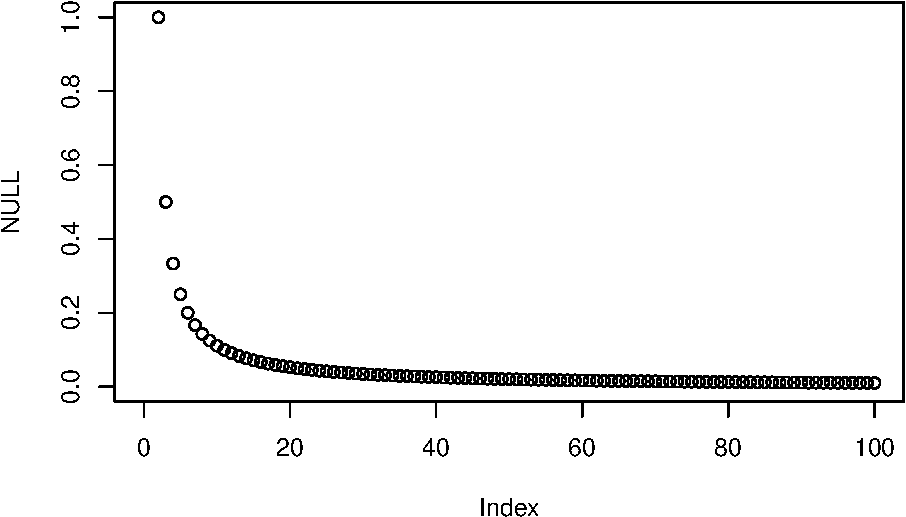
\includegraphics{Lab4_Matrix_Algebra_Functions_files/figure-latex/break1-1.pdf}

Example: make the Fibonacci series less than 300:

\begin{Shaded}
\begin{Highlighting}[]
\CommentTok{# Example: make the Fibonacci series less than 300}
\NormalTok{Fib1 <-}\StringTok{ }\DecValTok{1}
\NormalTok{Fib2 <-}\StringTok{ }\DecValTok{1}
\NormalTok{Fibonacci <-}\StringTok{ }\KeywordTok{c}\NormalTok{(}\DecValTok{0}\NormalTok{, Fib2)}
\ControlFlowTok{repeat}\NormalTok{\{}
\NormalTok{  Fibonacci <-}\StringTok{ }\KeywordTok{c}\NormalTok{(Fibonacci, Fib2)}
\NormalTok{  oldFib2 <-}\StringTok{ }\NormalTok{Fib2}
\NormalTok{  Fib2<-Fib1 }\OperatorTok{+}\StringTok{ }\NormalTok{Fib2}
\NormalTok{  Fib1 <-}\StringTok{ }\NormalTok{oldFib2}
  \ControlFlowTok{if}\NormalTok{ (Fib2 }\OperatorTok{>}\StringTok{ }\DecValTok{300}\NormalTok{) \{}\ControlFlowTok{break}\NormalTok{\}}
\NormalTok{\}}
\NormalTok{Fibonacci}
\end{Highlighting}
\end{Shaded}

\begin{verbatim}
##  [1]   0   1   1   2   3   5   8  13  21  34  55  89 144 233
\end{verbatim}

**\url{Tip:**} Save your files before running any repeat. \emph{Better
yet\ldots{}\textbf{don't} use repeat.} You should write for-loops that
can stop on their own.

\clearpage

\subsection{\texorpdfstring{\texttt{while()}}{while()}}\label{while}

A \texttt{while()} loop is just a repeat, where the
\texttt{if(condition)\{break\}} is specified at the top. Similar to the
above:

\begin{Shaded}
\begin{Highlighting}[]
\KeywordTok{plot}\NormalTok{(}\OtherTok{NULL}\NormalTok{, }\DataTypeTok{xlim=}\KeywordTok{c}\NormalTok{(}\DecValTok{0}\NormalTok{,}\DecValTok{100}\NormalTok{), }\DataTypeTok{ylim=}\KeywordTok{c}\NormalTok{(}\DecValTok{0}\NormalTok{,}\DecValTok{1}\NormalTok{))}
\NormalTok{x <-}\StringTok{ }\DecValTok{0}
\ControlFlowTok{while}\NormalTok{(x }\OperatorTok{<}\StringTok{ }\DecValTok{100}\NormalTok{) \{}
\NormalTok{  y <-}\StringTok{ }\DecValTok{1}\OperatorTok{/}\NormalTok{x}
\NormalTok{  x <-}\StringTok{ }\NormalTok{x}\OperatorTok{+}\DecValTok{1}
  \KeywordTok{points}\NormalTok{(x,y)}
\NormalTok{\}}
\end{Highlighting}
\end{Shaded}

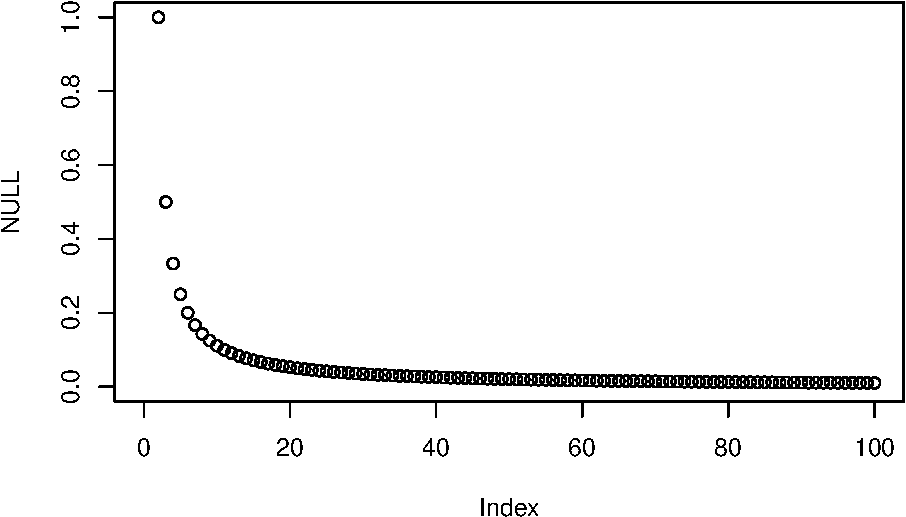
\includegraphics{Lab4_Matrix_Algebra_Functions_files/figure-latex/while1-1.pdf}

\begin{Shaded}
\begin{Highlighting}[]
\CommentTok{# Example 2}
\NormalTok{Fib1 <-}\StringTok{ }\DecValTok{1}
\NormalTok{Fib2 <-}\StringTok{ }\DecValTok{1}
\NormalTok{Fibonacci <-}\StringTok{ }\KeywordTok{c}\NormalTok{(}\DecValTok{0}\NormalTok{, Fib2)}
\ControlFlowTok{while}\NormalTok{(Fib2 }\OperatorTok{<=}\StringTok{ }\DecValTok{300}\NormalTok{)\{}
\NormalTok{  Fibonacci <-}\StringTok{ }\KeywordTok{c}\NormalTok{(Fibonacci, Fib2)}
\NormalTok{  oldFib2 <-}\StringTok{ }\NormalTok{Fib2}
\NormalTok{  Fib2 <-}\StringTok{ }\NormalTok{Fib1 }\OperatorTok{+}\StringTok{ }\NormalTok{Fib2}
\NormalTok{  Fib1 <-}\StringTok{ }\NormalTok{oldFib2}
\NormalTok{\}}
\NormalTok{Fibonacci}
\end{Highlighting}
\end{Shaded}

\begin{verbatim}
##  [1]   0   1   1   2   3   5   8  13  21  34  55  89 144 233
\end{verbatim}

\subsubsection{Example, using the Fearon and Laitin
data}\label{example-using-the-fearon-and-laitin-data}

Let's say we want to calculate the average number of civil-wars onsets
for each level of democratization (polity2)

\begin{Shaded}
\begin{Highlighting}[]
\KeywordTok{library}\NormalTok{(foreign)}
\NormalTok{civilw <-}\StringTok{ }\KeywordTok{read.dta}\NormalTok{(}\StringTok{"repdata.dta"}\NormalTok{)}
\NormalTok{democracy <-}\StringTok{ }\KeywordTok{min}\NormalTok{(civilw}\OperatorTok{$}\NormalTok{polity2, }\DataTypeTok{na.rm=}\NormalTok{T)}
\NormalTok{output_vector <-}\StringTok{ }\OtherTok{NULL}
\NormalTok{index <-}\StringTok{ }\DecValTok{1}
\ControlFlowTok{while}\NormalTok{(democracy }\OperatorTok{<=}\StringTok{ }\KeywordTok{max}\NormalTok{(civilw}\OperatorTok{$}\NormalTok{polity2, }\DataTypeTok{na.rm=}\NormalTok{T))\{}
\NormalTok{  output_vector[index] <-}\StringTok{ }\KeywordTok{mean}\NormalTok{(civilw}\OperatorTok{$}\NormalTok{onset[civilw}\OperatorTok{$}\NormalTok{polity2 }\OperatorTok{==}\StringTok{ }\NormalTok{democracy], }\DataTypeTok{na.rm=}\NormalTok{T)}
\NormalTok{  democracy <-}\StringTok{ }\NormalTok{democracy }\OperatorTok{+}\StringTok{ }\DecValTok{1} \CommentTok{# DON'T FORGET THIS LINE OR YOU WILL BE IN AN }\RegionMarkerTok{END}\CommentTok{LESS LOOP}
\NormalTok{  index <-}\StringTok{ }\NormalTok{index }\OperatorTok{+}\StringTok{ }\DecValTok{1} \CommentTok{# this line is needed to index forward}
\NormalTok{\}}
\NormalTok{output_vector}\OperatorTok{*}\DecValTok{100} \CommentTok{# civil wars start this percent of the time at each level of democracy}
\end{Highlighting}
\end{Shaded}

\begin{verbatim}
##  [1]  0.5235602  1.5015015  1.3623978  1.4115899  1.9543974  4.6875000
##  [7]  3.4782609  1.6574586  0.9523810  2.0833333 10.7784431  4.1095890
## [13]  1.8518519  3.4482759  3.2051282  3.0303030  1.1299435  1.4492754
## [19]  2.1875000  0.6993007  0.3289474
\end{verbatim}

\begin{Shaded}
\begin{Highlighting}[]
\KeywordTok{plot}\NormalTok{(}\KeywordTok{c}\NormalTok{(}\KeywordTok{min}\NormalTok{(civilw}\OperatorTok{$}\NormalTok{polity2, }\DataTypeTok{na.rm=}\NormalTok{T)}\OperatorTok{:}\KeywordTok{max}\NormalTok{(civilw}\OperatorTok{$}\NormalTok{polity2, }\DataTypeTok{na.rm=}\NormalTok{T)), output_vector}\OperatorTok{*}\DecValTok{100}\NormalTok{,}
     \DataTypeTok{xlab=}\StringTok{"Polity Scores"}\NormalTok{, }\DataTypeTok{ylab=}\StringTok{"% Civil War Onset"}\NormalTok{)}
\end{Highlighting}
\end{Shaded}

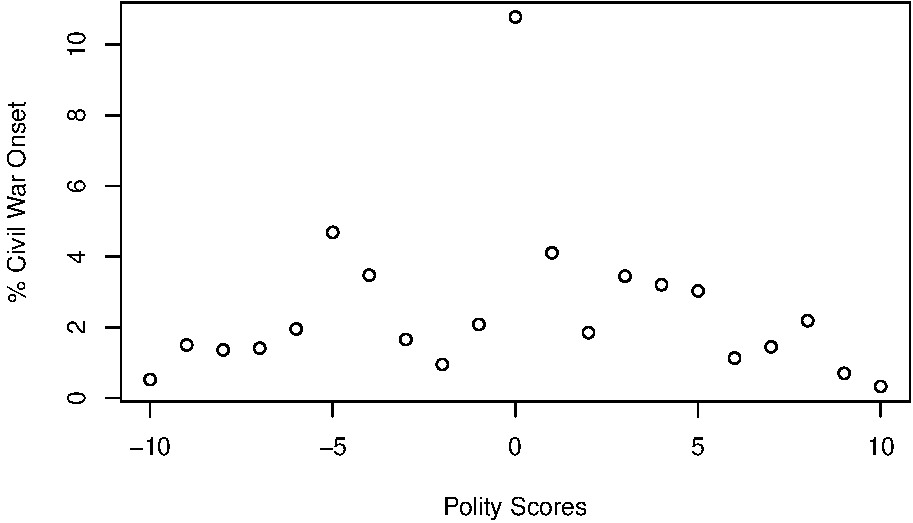
\includegraphics{Lab4_Matrix_Algebra_Functions_files/figure-latex/FL1-1.pdf}

In general, this is a pretty hack-y way to calculate this, and you're
better off using something like \texttt{data.table}, as discussed in lab
2.

\clearpage

\subsection{\texorpdfstring{for-loops,
\texttt{next()}}{for-loops, next()}}\label{for-loops-next}

The while loop still requires a lot of attention to indexing. Also
\ldots{} in many instances all we want to do is increment by 1. So
programmers put together a ``for loop.''

\texttt{for\ (name\ in\ vector)\ \{execute\ these\ commands\ on\ each\ value\ of\ the\ vector\}}
whatever you put into the name slot will become a ``local'' variable

\begin{Shaded}
\begin{Highlighting}[]
\ControlFlowTok{for}\NormalTok{ (monkey }\ControlFlowTok{in} \KeywordTok{c}\NormalTok{(}\StringTok{"spider"}\NormalTok{, }\StringTok{"howler"}\NormalTok{, }\StringTok{"wurst"}\NormalTok{))\{}\KeywordTok{print}\NormalTok{(monkey)\}}
\end{Highlighting}
\end{Shaded}

\begin{verbatim}
## [1] "spider"
## [1] "howler"
## [1] "wurst"
\end{verbatim}

\begin{Shaded}
\begin{Highlighting}[]
\CommentTok{# or more commonly}
\ControlFlowTok{for}\NormalTok{ (i }\ControlFlowTok{in} \DecValTok{1}\OperatorTok{:}\DecValTok{20}\NormalTok{)\{}
  \KeywordTok{print}\NormalTok{(i)}
\NormalTok{\}}
\end{Highlighting}
\end{Shaded}

\begin{verbatim}
## [1] 1
## [1] 2
## [1] 3
## [1] 4
## [1] 5
## [1] 6
## [1] 7
## [1] 8
## [1] 9
## [1] 10
## [1] 11
## [1] 12
## [1] 13
## [1] 14
## [1] 15
## [1] 16
## [1] 17
## [1] 18
## [1] 19
## [1] 20
\end{verbatim}

\subsubsection{Example of for-loops}\label{example-of-for-loops}

\begin{Shaded}
\begin{Highlighting}[]
\KeywordTok{plot}\NormalTok{(}\OtherTok{NULL}\NormalTok{, }\DataTypeTok{xlim=}\KeywordTok{c}\NormalTok{(}\DecValTok{0}\NormalTok{,}\DecValTok{100}\NormalTok{), }\DataTypeTok{ylim=}\KeywordTok{c}\NormalTok{(}\DecValTok{0}\NormalTok{,}\DecValTok{1}\NormalTok{))}
\ControlFlowTok{for}\NormalTok{ (i }\ControlFlowTok{in} \DecValTok{0}\OperatorTok{:}\DecValTok{100}\NormalTok{)\{}\KeywordTok{points}\NormalTok{(i, }\DecValTok{1}\OperatorTok{/}\NormalTok{i)\}}
\end{Highlighting}
\end{Shaded}

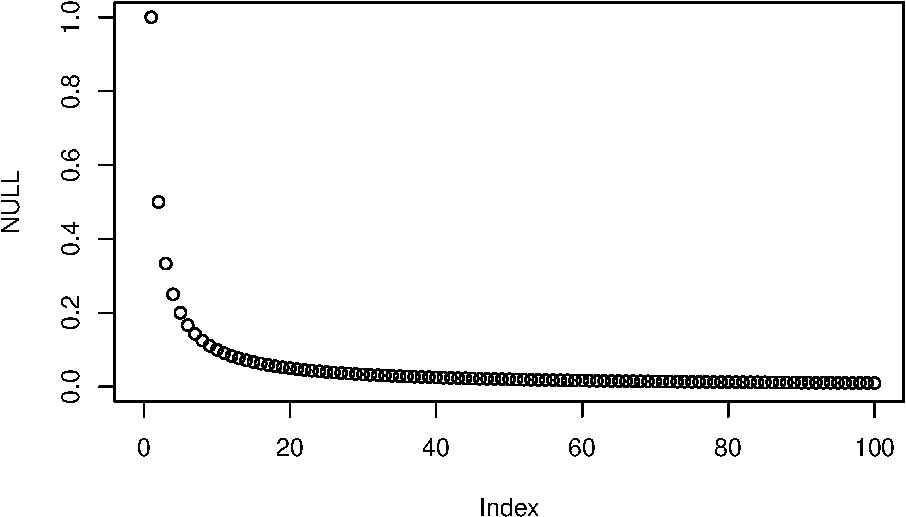
\includegraphics{Lab4_Matrix_Algebra_Functions_files/figure-latex/for2-1.pdf}

\begin{Shaded}
\begin{Highlighting}[]
\KeywordTok{plot}\NormalTok{(}\OtherTok{NULL}\NormalTok{, }\DataTypeTok{xlim=}\KeywordTok{c}\NormalTok{(}\DecValTok{0}\NormalTok{,}\DecValTok{11}\NormalTok{), }\DataTypeTok{ylim=}\KeywordTok{c}\NormalTok{(}\DecValTok{0}\NormalTok{,}\DecValTok{11}\NormalTok{))}
\ControlFlowTok{for}\NormalTok{(i }\ControlFlowTok{in} \DecValTok{1}\OperatorTok{:}\DecValTok{10}\NormalTok{)\{}
  \KeywordTok{abline}\NormalTok{(}\DataTypeTok{v=}\NormalTok{i)}
  \KeywordTok{abline}\NormalTok{(}\DataTypeTok{h=}\NormalTok{i)}
\NormalTok{\}}
\end{Highlighting}
\end{Shaded}

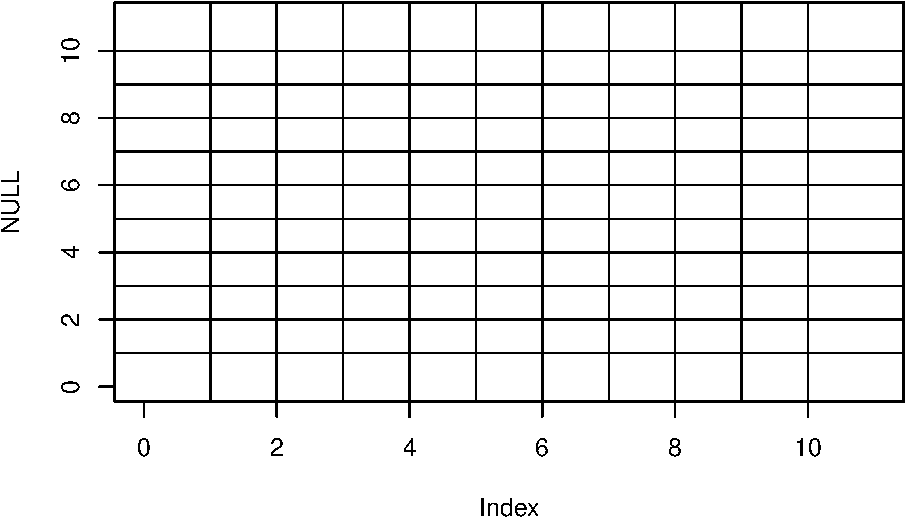
\includegraphics{Lab4_Matrix_Algebra_Functions_files/figure-latex/for2-2.pdf}

\begin{Shaded}
\begin{Highlighting}[]
\NormalTok{output <-}\StringTok{ }\OtherTok{NULL}
\ControlFlowTok{for}\NormalTok{(i }\ControlFlowTok{in} \DecValTok{1}\OperatorTok{:}\DecValTok{20}\NormalTok{)\{}
\NormalTok{  output[i] <-}\StringTok{ }\DecValTok{0}\OperatorTok{+}\NormalTok{i}
\NormalTok{\}}
\end{Highlighting}
\end{Shaded}

\begin{Shaded}
\begin{Highlighting}[]
\KeywordTok{library}\NormalTok{(foreign)}
\NormalTok{civilw <-}\StringTok{ }\KeywordTok{read.dta}\NormalTok{(}\StringTok{"repdata.dta"}\NormalTok{)}
\NormalTok{output_vector <-}\StringTok{ }\OtherTok{NULL} \CommentTok{# Still need to instantiate the variable or you cannot index it}
\NormalTok{democracy <-}\StringTok{ }\KeywordTok{sort}\NormalTok{(}\KeywordTok{unique}\NormalTok{(civilw}\OperatorTok{$}\NormalTok{polity2))}
\ControlFlowTok{for}\NormalTok{ (i }\ControlFlowTok{in} \KeywordTok{min}\NormalTok{(democracy)}\OperatorTok{:}\KeywordTok{max}\NormalTok{(democracy))\{}
\NormalTok{  output_vector <-}\StringTok{ }\KeywordTok{c}\NormalTok{(output_vector, }\KeywordTok{mean}\NormalTok{(civilw}\OperatorTok{$}\NormalTok{onset[civilw}\OperatorTok{$}\NormalTok{polity2 }\OperatorTok{==}\StringTok{ }\NormalTok{democracy[i}\OperatorTok{+}\DecValTok{11}\NormalTok{]], }\DataTypeTok{na.rm=}\NormalTok{T)}\OperatorTok{*}\DecValTok{100}\NormalTok{)}
\NormalTok{\}}
\KeywordTok{plot}\NormalTok{(}\KeywordTok{c}\NormalTok{(}\KeywordTok{min}\NormalTok{(democracy)}\OperatorTok{:}\KeywordTok{max}\NormalTok{(democracy)),output_vector,}
     \DataTypeTok{xlab=}\StringTok{"Polity Scores"}\NormalTok{, }\DataTypeTok{ylab=}\StringTok{"% civil War Onset"}\NormalTok{)}
\end{Highlighting}
\end{Shaded}

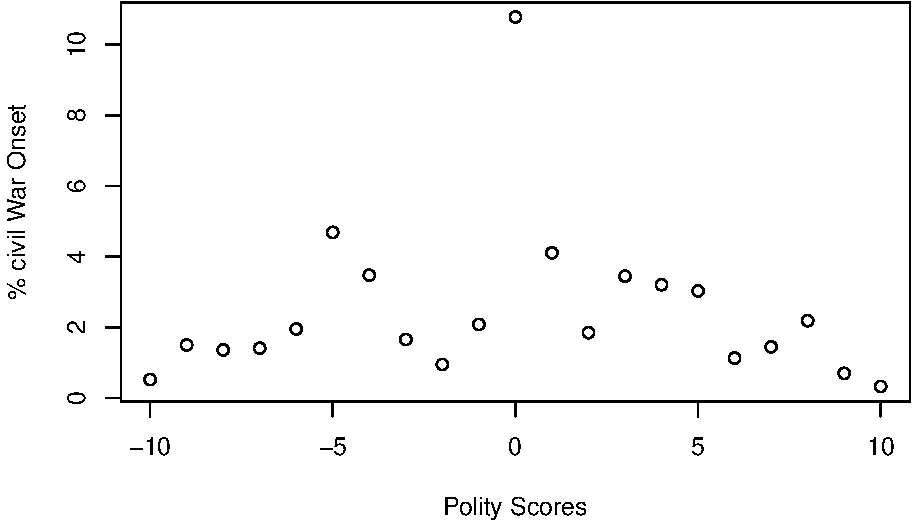
\includegraphics{Lab4_Matrix_Algebra_Functions_files/figure-latex/for3-1.pdf}

Sometimes you might not want to execute the commands for every element
in the vector use the next command to skip (you can also use the break)

\begin{Shaded}
\begin{Highlighting}[]
\NormalTok{some_odds <-}\StringTok{ }\OtherTok{NULL}
\ControlFlowTok{for}\NormalTok{ (i }\ControlFlowTok{in} \DecValTok{1}\OperatorTok{:}\DecValTok{200}\NormalTok{)\{}
  \ControlFlowTok{if}\NormalTok{ (i}\OperatorTok\DecValTok{2} \OperatorTok{!=}\StringTok{ }\DecValTok{0}\NormalTok{) \{}
\NormalTok{    some_odds<-}\KeywordTok{c}\NormalTok{(some_odds, i)}
\NormalTok{  \} }\ControlFlowTok{else}\NormalTok{ \{ }\ControlFlowTok{next}\NormalTok{ \}}
\NormalTok{\}}
\NormalTok{some_odds}
\end{Highlighting}
\end{Shaded}

\begin{verbatim}
##   [1]   1   3   5   7   9  11  13  15  17  19  21  23  25  27  29  31  33
##  [18]  35  37  39  41  43  45  47  49  51  53  55  57  59  61  63  65  67
##  [35]  69  71  73  75  77  79  81  83  85  87  89  91  93  95  97  99 101
##  [52] 103 105 107 109 111 113 115 117 119 121 123 125 127 129 131 133 135
##  [69] 137 139 141 143 145 147 149 151 153 155 157 159 161 163 165 167 169
##  [86] 171 173 175 177 179 181 183 185 187 189 191 193 195 197 199
\end{verbatim}

\clearpage

\subsection{Functions}\label{functions}

We have been using functions this whole time, but we can also make our
own. This both helps you keep your code organized, and helps you better
understand other people's functions. In particular, functions can be
helpful if you have a repetitive serious of tasks to perform on your
data.

\subsubsection{Example:}\label{example}

Here are three ways to write the same function:

\begin{Shaded}
\begin{Highlighting}[]
\NormalTok{my_function1 <-}\StringTok{ }\ControlFlowTok{function}\NormalTok{(x)\{ }\CommentTok{# take in a value of x}
\NormalTok{  y<-x}\OperatorTok{^}\DecValTok{2}\OperatorTok{+}\DecValTok{3}\OperatorTok{*}\NormalTok{x}\OperatorTok{-}\DecValTok{2} \CommentTok{# conduct some set of operations using the input values}
  \KeywordTok{return}\NormalTok{(y) }\CommentTok{# return some value. In this case we are returning a simple numeric value}
\NormalTok{\}}

\NormalTok{my_function2 <-}\StringTok{ }\ControlFlowTok{function}\NormalTok{(x)\{}
\NormalTok{  x}\OperatorTok{^}\DecValTok{2}\OperatorTok{+}\DecValTok{3}\OperatorTok{*}\NormalTok{x}\OperatorTok{-}\DecValTok{2} \CommentTok{# we don't have to specify a return}
\NormalTok{\}}

\NormalTok{my_function3 <-}\StringTok{ }\ControlFlowTok{function}\NormalTok{(x) x}\OperatorTok{^}\DecValTok{2}\OperatorTok{+}\DecValTok{3}\OperatorTok{*}\NormalTok{x}\OperatorTok{-}\DecValTok{2} \CommentTok{# for simple functions, we don't even need brackets}


\KeywordTok{my_function1}\NormalTok{(}\KeywordTok{c}\NormalTok{(}\DecValTok{1}\OperatorTok{:}\DecValTok{20}\NormalTok{))}
\end{Highlighting}
\end{Shaded}

\begin{verbatim}
##  [1]   2   8  16  26  38  52  68  86 106 128 152 178 206 236 268 302 338
## [18] 376 416 458
\end{verbatim}

\begin{Shaded}
\begin{Highlighting}[]
\KeywordTok{my_function2}\NormalTok{(}\KeywordTok{c}\NormalTok{(}\DecValTok{1}\OperatorTok{:}\DecValTok{20}\NormalTok{))}
\end{Highlighting}
\end{Shaded}

\begin{verbatim}
##  [1]   2   8  16  26  38  52  68  86 106 128 152 178 206 236 268 302 338
## [18] 376 416 458
\end{verbatim}

\begin{Shaded}
\begin{Highlighting}[]
\KeywordTok{my_function3}\NormalTok{(}\KeywordTok{c}\NormalTok{(}\DecValTok{1}\OperatorTok{:}\DecValTok{20}\NormalTok{))}
\end{Highlighting}
\end{Shaded}

\begin{verbatim}
##  [1]   2   8  16  26  38  52  68  86 106 128 152 178 206 236 268 302 338
## [18] 376 416 458
\end{verbatim}

1 or 2 are the preferred ways to write functions, for the same reason we
used braces with \texttt{if()} and \texttt{else()}: they make code more
legible.

Functions are just another object. We can define the functions using: 1.
The word \texttt{function} 2. A pair of round parentheses \texttt{()}
which enclose the argument list. The list may be empty. 3. A single
statement, or a sequence of statements enclosed in curly braces
\texttt{\{\ \}}.

Sometimes a function will return a value, but other times it will just
execute a command.

\begin{Shaded}
\begin{Highlighting}[]
\NormalTok{mad_libs <-}\StringTok{ }\ControlFlowTok{function}\NormalTok{(noun, location, proper_noun, activity)\{}
  \KeywordTok{print}\NormalTok{(}\KeywordTok{paste}\NormalTok{(}\StringTok{"One day, I was looking all over for my"}\NormalTok{, noun))}
  \KeywordTok{print}\NormalTok{(}\KeywordTok{paste}\NormalTok{(}\StringTok{"I decided I must have left it at the"}\NormalTok{, location))}
  \KeywordTok{print}\NormalTok{(}\KeywordTok{paste}\NormalTok{(}\StringTok{"When I got there, I found"}\NormalTok{, proper_noun, }\StringTok{"using my"}\NormalTok{, noun, }\StringTok{"to"}\NormalTok{, activity))}
\NormalTok{\}}
\KeywordTok{mad_libs}\NormalTok{(}\StringTok{"baseball"}\NormalTok{, }\StringTok{"lake house"}\NormalTok{, }\StringTok{"Jan Pierskalla"}\NormalTok{, }\StringTok{"eat pudding"}\NormalTok{)}
\end{Highlighting}
\end{Shaded}

\begin{verbatim}
## [1] "One day, I was looking all over for my baseball"
## [1] "I decided I must have left it at the lake house"
## [1] "When I got there, I found Jan Pierskalla using my baseball to eat pudding"
\end{verbatim}

\begin{Shaded}
\begin{Highlighting}[]
\NormalTok{sqrt_plotter <-}\StringTok{ }\ControlFlowTok{function}\NormalTok{(x)\{}
  \KeywordTok{plot}\NormalTok{(x, }\KeywordTok{sqrt}\NormalTok{(x))}
\NormalTok{\}}
\KeywordTok{sqrt_plotter}\NormalTok{(}\DecValTok{1}\OperatorTok{:}\DecValTok{10}\NormalTok{)}
\end{Highlighting}
\end{Shaded}

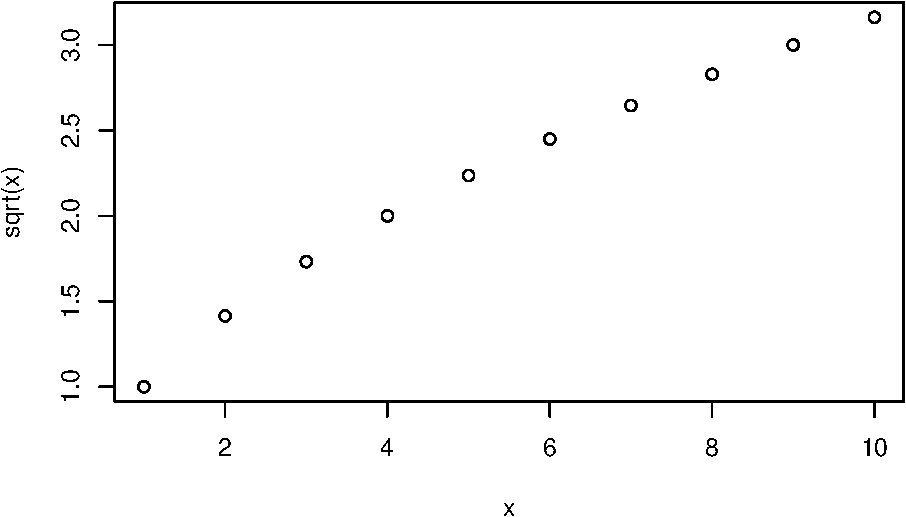
\includegraphics{Lab4_Matrix_Algebra_Functions_files/figure-latex/function3-1.pdf}

Other times we will want to return a value

\begin{Shaded}
\begin{Highlighting}[]
\NormalTok{my_abs <-}\StringTok{ }\ControlFlowTok{function}\NormalTok{(x)\{}
  \KeywordTok{ifelse}\NormalTok{(x}\OperatorTok{<=}\DecValTok{0}\NormalTok{, }\OperatorTok{-}\DecValTok{1}\OperatorTok{*}\NormalTok{x, x)}
\NormalTok{\}}
\KeywordTok{my_abs}\NormalTok{(}\KeywordTok{c}\NormalTok{(}\OperatorTok{-}\DecValTok{1}\NormalTok{,}\DecValTok{2}\NormalTok{,}\DecValTok{3}\NormalTok{,}\OperatorTok{-}\DecValTok{4}\NormalTok{,}\DecValTok{5}\NormalTok{))}
\end{Highlighting}
\end{Shaded}

\begin{verbatim}
## [1] 1 2 3 4 5
\end{verbatim}

You can set default values for some of your arguments or all of them:

\begin{Shaded}
\begin{Highlighting}[]
\NormalTok{gaga_equation <-}\StringTok{ }\ControlFlowTok{function}\NormalTok{(}\DataTypeTok{num_rah=}\DecValTok{2}\NormalTok{, }\DataTypeTok{num_ah=}\DecValTok{3}\NormalTok{, }\DataTypeTok{num_ga=}\DecValTok{2}\NormalTok{, }\DataTypeTok{num_la=}\DecValTok{2}\NormalTok{)\{}
\NormalTok{  rahs<-}\KeywordTok{paste}\NormalTok{(}\KeywordTok{rep}\NormalTok{(}\StringTok{"RAH"}\NormalTok{, num_rah), }\DataTypeTok{collapse=}\StringTok{", "}\NormalTok{)}
\NormalTok{  ahs<-}\KeywordTok{paste}\NormalTok{(}\KeywordTok{rep}\NormalTok{(}\StringTok{"AH"}\NormalTok{, num_ah), }\DataTypeTok{collapse=}\StringTok{", "}\NormalTok{)}
\NormalTok{  gas<-}\KeywordTok{paste}\NormalTok{(}\KeywordTok{rep}\NormalTok{(}\StringTok{"GA"}\NormalTok{, num_ga), }\DataTypeTok{collapse=}\StringTok{", "}\NormalTok{)}
\NormalTok{  las<-}\KeywordTok{paste}\NormalTok{(}\KeywordTok{rep}\NormalTok{(}\StringTok{"LA"}\NormalTok{, num_la), }\DataTypeTok{collapse=}\StringTok{", "}\NormalTok{)}
  \KeywordTok{paste}\NormalTok{(rahs, }\StringTok{","}\NormalTok{, ahs,  }\StringTok{"!  ROMA, ROMAMA!"}\NormalTok{, gas,}\StringTok{","}\NormalTok{, las)}
\NormalTok{\}}
\KeywordTok{gaga_equation}\NormalTok{()}
\end{Highlighting}
\end{Shaded}

\begin{verbatim}
## [1] "RAH, RAH , AH, AH, AH !  ROMA, ROMAMA! GA, GA , LA, LA"
\end{verbatim}

\begin{Shaded}
\begin{Highlighting}[]
\KeywordTok{gaga_equation}\NormalTok{(}\DataTypeTok{num_rah=}\DecValTok{5}\NormalTok{)}
\end{Highlighting}
\end{Shaded}

\begin{verbatim}
## [1] "RAH, RAH, RAH, RAH, RAH , AH, AH, AH !  ROMA, ROMAMA! GA, GA , LA, LA"
\end{verbatim}

Note that variables created within the function are NOT in the global
environment, they don't exist ``outside'' of the function, and cease to
exist when the function stops running. In the \texttt{gaga\_equation},
you can't call \texttt{rahs} outside of the function.

Many of the functions you will write or work with will return lists,
like the \texttt{summary} command.

\begin{Shaded}
\begin{Highlighting}[]
\KeywordTok{library}\NormalTok{(foreign)}
\NormalTok{civilw <-}\StringTok{ }\KeywordTok{read.dta}\NormalTok{(}\StringTok{"repdata.dta"}\NormalTok{)}


\NormalTok{my_summary <-}\StringTok{ }\ControlFlowTok{function}\NormalTok{(varname, }\DataTypeTok{data=}\NormalTok{civilw)\{}
  \KeywordTok{attach}\NormalTok{(civilw)}
\NormalTok{  this_mean <-}\StringTok{ }\KeywordTok{mean}\NormalTok{(varname, }\DataTypeTok{na.rm=}\NormalTok{T)}
\NormalTok{  this_var <-}\StringTok{ }\KeywordTok{var}\NormalTok{(varname, }\DataTypeTok{na.rm=}\NormalTok{T)}
\NormalTok{  this_quant <-}\StringTok{ }\KeywordTok{quantile}\NormalTok{(varname, }\KeywordTok{c}\NormalTok{(.}\DecValTok{025}\NormalTok{, .}\DecValTok{25}\NormalTok{, .}\DecValTok{5}\NormalTok{, .}\DecValTok{75}\NormalTok{, .}\DecValTok{975}\NormalTok{), }\DataTypeTok{na.rm=}\NormalTok{T)}
  \KeywordTok{detach}\NormalTok{(civilw)}
  \KeywordTok{return}\NormalTok{(}\KeywordTok{list}\NormalTok{(}\DataTypeTok{mean=}\NormalTok{this_mean, }\DataTypeTok{variance=}\NormalTok{this_var, }\DataTypeTok{quantiles=}\NormalTok{this_quant))}
\NormalTok{\}}
\KeywordTok{my_summary}\NormalTok{(polity2)}
\end{Highlighting}
\end{Shaded}

\begin{verbatim}
## $mean
## [1] -0.4130136
## 
## $variance
## [1] 56.62469
## 
## $quantiles
##  2.5%   25%   50%   75% 97.5% 
##   -10    -7    -3     8    10
\end{verbatim}

\begin{Shaded}
\begin{Highlighting}[]
\NormalTok{polity2_summary <-}\StringTok{ }\KeywordTok{my_summary}\NormalTok{(polity2)}
\KeywordTok{str}\NormalTok{(polity2_summary)}
\end{Highlighting}
\end{Shaded}

\begin{verbatim}
## List of 3
##  $ mean     : num -0.413
##  $ variance : num 56.6
##  $ quantiles: Named num [1:5] -10 -7 -3 8 10
##   ..- attr(*, "names")= chr [1:5] "2.5%" "25%" "50%" "75%" ...
\end{verbatim}

\subsection{2.6: A note on classes}\label{a-note-on-classes}

If you run \texttt{?lm}, doesn't it look like it is returning a list?

\begin{Shaded}
\begin{Highlighting}[]
\KeywordTok{library}\NormalTok{(foreign)}
\NormalTok{civilw <-}\StringTok{ }\KeywordTok{read.dta}\NormalTok{(}\StringTok{"repdata.dta"}\NormalTok{)}

\NormalTok{lm1 <-}\StringTok{ }\KeywordTok{lm}\NormalTok{(polity2 }\OperatorTok{~}\StringTok{ }\NormalTok{gdpen, }\DataTypeTok{data=}\NormalTok{civilw)}
\KeywordTok{str}\NormalTok{(lm1) }\CommentTok{# it looks like a really complicated list}
\end{Highlighting}
\end{Shaded}

\begin{verbatim}
## List of 13
##  $ coefficients : Named num [1:2] -2.743 0.655
##   ..- attr(*, "names")= chr [1:2] "(Intercept)" "gdpen"
##  $ residuals    : Named num [1:6343] 7.75 7.73 7.49 7.33 7.48 ...
##   ..- attr(*, "names")= chr [1:6343] "1" "2" "3" "4" ...
##  $ effects      : Named num [1:6343] 26.17 -228.39 7.3 7.13 7.29 ...
##   ..- attr(*, "names")= chr [1:6343] "(Intercept)" "gdpen" "" "" ...
##  $ rank         : int 2
##  $ fitted.values: Named num [1:6343] 2.25 2.27 2.51 2.67 2.52 ...
##   ..- attr(*, "names")= chr [1:6343] "1" "2" "3" "4" ...
##  $ assign       : int [1:2] 0 1
##  $ qr           :List of 5
##   ..$ qr   : num [1:6343, 1:2] -79.643 0.0126 0.0126 0.0126 0.0126 ...
##   .. ..- attr(*, "dimnames")=List of 2
##   .. .. ..$ : chr [1:6343] "1" "2" "3" "4" ...
##   .. .. ..$ : chr [1:2] "(Intercept)" "gdpen"
##   .. ..- attr(*, "assign")= int [1:2] 0 1
##   ..$ qraux: num [1:2] 1.01 1.01
##   ..$ pivot: int [1:2] 1 2
##   ..$ tol  : num 1e-07
##   ..$ rank : int 2
##   ..- attr(*, "class")= chr "qr"
##  $ df.residual  : int 6341
##  $ na.action    :Class 'omit'  Named int [1:267] 111 158 159 160 161 162 163 164 165 166 ...
##   .. ..- attr(*, "names")= chr [1:267] "111" "158" "159" "160" ...
##  $ xlevels      : Named list()
##  $ call         : language lm(formula = polity2 ~ gdpen, data = civilw)
##  $ terms        :Classes 'terms', 'formula'  language polity2 ~ gdpen
##   .. ..- attr(*, "variables")= language list(polity2, gdpen)
##   .. ..- attr(*, "factors")= int [1:2, 1] 0 1
##   .. .. ..- attr(*, "dimnames")=List of 2
##   .. .. .. ..$ : chr [1:2] "polity2" "gdpen"
##   .. .. .. ..$ : chr "gdpen"
##   .. ..- attr(*, "term.labels")= chr "gdpen"
##   .. ..- attr(*, "order")= int 1
##   .. ..- attr(*, "intercept")= int 1
##   .. ..- attr(*, "response")= int 1
##   .. ..- attr(*, ".Environment")=<environment: R_GlobalEnv> 
##   .. ..- attr(*, "predvars")= language list(polity2, gdpen)
##   .. ..- attr(*, "dataClasses")= Named chr [1:2] "numeric" "numeric"
##   .. .. ..- attr(*, "names")= chr [1:2] "polity2" "gdpen"
##  $ model        :'data.frame':   6343 obs. of  2 variables:
##   ..$ polity2: num [1:6343] 10 10 10 10 10 10 10 10 10 10 ...
##   ..$ gdpen  : num [1:6343] 7.63 7.65 8.02 8.27 8.04 ...
##   ..- attr(*, "terms")=Classes 'terms', 'formula'  language polity2 ~ gdpen
##   .. .. ..- attr(*, "variables")= language list(polity2, gdpen)
##   .. .. ..- attr(*, "factors")= int [1:2, 1] 0 1
##   .. .. .. ..- attr(*, "dimnames")=List of 2
##   .. .. .. .. ..$ : chr [1:2] "polity2" "gdpen"
##   .. .. .. .. ..$ : chr "gdpen"
##   .. .. ..- attr(*, "term.labels")= chr "gdpen"
##   .. .. ..- attr(*, "order")= int 1
##   .. .. ..- attr(*, "intercept")= int 1
##   .. .. ..- attr(*, "response")= int 1
##   .. .. ..- attr(*, ".Environment")=<environment: R_GlobalEnv> 
##   .. .. ..- attr(*, "predvars")= language list(polity2, gdpen)
##   .. .. ..- attr(*, "dataClasses")= Named chr [1:2] "numeric" "numeric"
##   .. .. .. ..- attr(*, "names")= chr [1:2] "polity2" "gdpen"
##   ..- attr(*, "na.action")=Class 'omit'  Named int [1:267] 111 158 159 160 161 162 163 164 165 166 ...
##   .. .. ..- attr(*, "names")= chr [1:267] "111" "158" "159" "160" ...
##  - attr(*, "class")= chr "lm"
\end{verbatim}

\begin{Shaded}
\begin{Highlighting}[]
\NormalTok{lm1[[}\DecValTok{1}\NormalTok{]] }\CommentTok{# it acts like a list}
\end{Highlighting}
\end{Shaded}

\begin{verbatim}
## (Intercept)       gdpen 
##  -2.7429009   0.6550537
\end{verbatim}

\begin{Shaded}
\begin{Highlighting}[]
\NormalTok{lm1}\OperatorTok{$}\NormalTok{coefficients}
\end{Highlighting}
\end{Shaded}

\begin{verbatim}
## (Intercept)       gdpen 
##  -2.7429009   0.6550537
\end{verbatim}

\begin{Shaded}
\begin{Highlighting}[]
\NormalTok{lm1[}\StringTok{"coefficients"}\NormalTok{]}
\end{Highlighting}
\end{Shaded}

\begin{verbatim}
## $coefficients
## (Intercept)       gdpen 
##  -2.7429009   0.6550537
\end{verbatim}

\begin{Shaded}
\begin{Highlighting}[]
\KeywordTok{class}\NormalTok{(lm1) }\CommentTok{# But it's not a list}
\end{Highlighting}
\end{Shaded}

\begin{verbatim}
## [1] "lm"
\end{verbatim}

This is an object in the ``lm'' class. In this case, it works mostly
like a list. Mostly this is because some functions will work differently
for objects of different classes

\begin{Shaded}
\begin{Highlighting}[]
\KeywordTok{print}\NormalTok{(lm1)}
\end{Highlighting}
\end{Shaded}

\begin{verbatim}
## 
## Call:
## lm(formula = polity2 ~ gdpen, data = civilw)
## 
## Coefficients:
## (Intercept)        gdpen  
##     -2.7429       0.6551
\end{verbatim}

\begin{Shaded}
\begin{Highlighting}[]
\CommentTok{# print(unclass(lm1)) # that's all of the raw data}
\end{Highlighting}
\end{Shaded}

R offers the ability to modify functions based on the class of an object

\begin{Shaded}
\begin{Highlighting}[]
\KeywordTok{methods}\NormalTok{(}\DataTypeTok{class =} \StringTok{"lm"}\NormalTok{) }\CommentTok{# these are functions that do something different for the class lm than they would for some different classes}
\end{Highlighting}
\end{Shaded}

\begin{verbatim}
##  [1] add1           alias          anova          case.names    
##  [5] coerce         confint        cooks.distance deviance      
##  [9] dfbeta         dfbetas        drop1          dummy.coef    
## [13] effects        extractAIC     family         formula       
## [17] hatvalues      influence      initialize     kappa         
## [21] labels         logLik         model.frame    model.matrix  
## [25] nobs           plot           predict        print         
## [29] proj           qr             residuals      rstandard     
## [33] rstudent       show           simulate       slotsFromS3   
## [37] summary        variable.names vcov          
## see '?methods' for accessing help and source code
\end{verbatim}

\begin{Shaded}
\begin{Highlighting}[]
\KeywordTok{methods}\NormalTok{(plot) }\CommentTok{# These are all the variants of the function plot.  For each of these classes of objects different sets of actual instructions are followed.}
\end{Highlighting}
\end{Shaded}

\begin{verbatim}
##  [1] plot.acf*           plot.data.frame*    plot.decomposed.ts*
##  [4] plot.default        plot.dendrogram*    plot.density*      
##  [7] plot.ecdf           plot.factor*        plot.formula*      
## [10] plot.function       plot.hclust*        plot.histogram*    
## [13] plot.HoltWinters*   plot.isoreg*        plot.lm*           
## [16] plot.medpolish*     plot.mlm*           plot.ppr*          
## [19] plot.prcomp*        plot.princomp*      plot.profile.nls*  
## [22] plot.raster*        plot.spec*          plot.stepfun       
## [25] plot.stl*           plot.table*         plot.ts            
## [28] plot.tskernel*      plot.TukeyHSD*     
## see '?methods' for accessing help and source code
\end{verbatim}

\section{2.7: A note on scope}\label{a-note-on-scope}

As we noted -- local variables are not written into the global
environment. Unless you are to the point where you are creating your own
namespaces (in which case you can explain all of that to me), you don't
need to worry much about scope except to understand that:

\begin{Shaded}
\begin{Highlighting}[]
\CommentTok{# What happens in the function, stays in the function}

\NormalTok{f <-}\ControlFlowTok{function}\NormalTok{() \{}
\NormalTok{  x <-}\StringTok{ }\DecValTok{1} \CommentTok{#local x}
  \KeywordTok{g}\NormalTok{()}
  \KeywordTok{return}\NormalTok{(x)}
\NormalTok{\}}
\NormalTok{g<-}\ControlFlowTok{function}\NormalTok{()\{}
\NormalTok{  x<-}\DecValTok{2} \CommentTok{# local x}
\NormalTok{\}}
\KeywordTok{f}\NormalTok{()}
\end{Highlighting}
\end{Shaded}

\begin{verbatim}
## [1] 1
\end{verbatim}

\begin{Shaded}
\begin{Highlighting}[]
\NormalTok{x<-}\DecValTok{3} \CommentTok{# global x}
\KeywordTok{f}\NormalTok{()}
\end{Highlighting}
\end{Shaded}

\begin{verbatim}
## [1] 1
\end{verbatim}

\begin{Shaded}
\begin{Highlighting}[]
\NormalTok{x}
\end{Highlighting}
\end{Shaded}

\begin{verbatim}
## [1] 3
\end{verbatim}

\begin{Shaded}
\begin{Highlighting}[]
\CommentTok{# HOWEVER: you can pass values downwards in a function chain}

\NormalTok{f <-}\ControlFlowTok{function}\NormalTok{() \{}
\NormalTok{  x<-}\StringTok{ }\DecValTok{1}
\NormalTok{  y<-}\StringTok{ }\KeywordTok{g}\NormalTok{(x)}
  \KeywordTok{return}\NormalTok{(}\KeywordTok{c}\NormalTok{(x, y))}
\NormalTok{\}}
\NormalTok{g<-}\ControlFlowTok{function}\NormalTok{(x)\{}
\NormalTok{  x}\OperatorTok{+}\DecValTok{2}
\NormalTok{\}}
\KeywordTok{f}\NormalTok{()}
\end{Highlighting}
\end{Shaded}

\begin{verbatim}
## [1] 1 3
\end{verbatim}


\end{document}
